\documentclass[10pt,a4paper]{article}
\usepackage[margin=20mm]{geometry}
\usepackage[T1]{fontenc}
\usepackage{lmodern}
\usepackage{amsmath,amssymb,graphicx,microtype,booktabs}
\usepackage{float}
\usepackage[font=small]{caption}
\usepackage[hidelinks]{hyperref}
\setlength{\parindent}{0pt}
\setlength{\parskip}{5pt}
\setlength{\textfloatsep}{12pt}
\newcommand{\fd}{f_\downarrow}
\newcommand{\fu}{f_\uparrow}
\newcommand{\fcs}{f_c}
\newcommand{\running}{\textit{(running)}}
\graphicspath{{../figures/}}
\begin{document}

\begin{center}
{\Large Depinning with inertia}\\[3pt]
{\small An elastic line in quenched disorder, driven by a constant force or a parabolic well}
\end{center}

\begin{quote}\small
\textbf{Abstract.}
An elastic line with mass $m$ and damping $\eta$ is driven through random-field or random-bond disorder; $M=\kappa m/(\eta L_c)^2$ measures inertia at the Larkin scale.
(i) For $M\lesssim0.5$ single jumps do not overshoot, the line visits the same metastable states as at $m=0$, and everything is qEW: same threshold, same avalanches event for event, $\tau=1.1\pm0.05$.
(ii) For $M\gtrsim5$ the threshold is the end of a hot, radiating sliding branch. A parameter-free closure predicts its minimum $f_{\min}(M)$, with $f_{\min}\propto m^{-3/10}$ (random field) and $m^{-5/14}$ (random bond) at large $M$.
(iii) Below $f_{\min}$ the line slides in patches, and the patchy state ends continuously at $f_\infty=(0.987\pm0.002)f_{\min}$ ($m=64$). There are no quenched rare regions, and spreading from a hot seed is superdiffusive ($z\simeq1.31\pm0.03$ in the largest run; $2/z=1.34$--$1.57$ across seeds and substrates): not directed percolation; conserved DP is not excluded.
(iv) The hot line is Edwards--Wilkinson ($\zeta=1/2$) with a scale-dependent temperature. A single-site (DMFT) theory with the one-loop disorder self-energy $\Sigma(\omega)$, one site in a self-consistent Gaussian bath, is closed and energy-conserving: with no input from simulation it predicts the flow curve within 1\%, $T_{\rm kin}$ within 3\% and the force noise $S_\xi(0)$ within 6\%. Its uniform hot branch stays stable below $f_\infty$: the end of sliding is a nucleation of pinned patches, not a spinodal.
(v) Ramp hysteresis is a finite-size, finite-time effect. Under slow displacement driving heavy lines stick and slip like a spring block whose kinetic friction is $f_{\min}$.
\end{quote}

\tableofcontents

%======================================================================
\section{Setup}
\label{sec:model}

\paragraph{Equation of motion.} The line has $L$ sites, periodic:
\begin{equation}
m\ddot u_i+\eta\dot u_i=\kappa\,(u_{i+1}+u_{i-1}-2u_i)+F_i(u_i)+f\;\big[\,+\,k_0(w-u_i)\big].
\label{eq:eom}
\end{equation}
Driving is either a constant force $f$ or a parabolic well $k_0(w-u_i)$ whose centre advances at rate $\dot w$.

\paragraph{Disorder.} $F_i(u)$ interpolates linearly between node values at integer $u$ ($r_f=1$), generated by a counter-based hash so the landscape is unbounded in $u$.
\begin{itemize}
\item \textbf{Random field (RF, default).} Nodes i.i.d.\ uniform on $[-A,A]$: $\langle F^2\rangle=2A^2/9$, $\Delta(x)=(A^2/3)M_4(x)$ ($M_4$ the cubic B-spline), $\hat\Delta(k)=(A^2/3)\,\mathrm{sinc}^4(k/2)$, $\hat\Delta(0)=A^2/3$.
\item \textbf{Random bond (RB).} Nodes are differences of i.i.d.\ values, so the potential is bounded: $\hat\Delta(k)=(A^2/3)(2-2\cos k)\,\mathrm{sinc}^4(k/2)$, $\hat\Delta(0)=0$, $\langle F^2\rangle=A^2/3$.
\end{itemize}

\paragraph{Scales.}
\begin{itemize}
\item Larkin length $L_c=(\kappa r_f/\langle F^2\rangle^{1/2})^{2/3}=1.65$ (RF, $A=1$); time $\tau_c=\eta L_c^2/\kappa$.
\item Inertial length $\ell_m=2\sqrt{\kappa m}/\eta$: modes with $q>1/\ell_m$ are underdamped and travel as sound at $c=\sqrt{\kappa/m}$.
\item Inertia parameter $M=\kappa m/(\eta^2L_c^2)=(\ell_m/2L_c)^2=0.37\,m$. Runs span $M=0.09$ to $2.4\times10^4$.
\end{itemize}

\paragraph{Units and numerics.} $\kappa=\eta=1$, $A=1$ unless stated. Time step: the exact damped update at frozen force, $v\leftarrow ve^{-\eta dt/m}+(F_{\rm tot}/\eta)(1-e^{-\eta dt/m})$, $u\leftarrow u+dt\,v$ (Euler at $m=0$), $dt=\min(0.4,\max(0.05,0.05\sqrt m))$; dividing $dt$ by 4 changes velocities by less than their errors.

\paragraph{Observables.} Static threshold $\fcs$ (largest $f$ with a stable configuration); ramp-down $\fd$ and ramp-up $\fu$ thresholds at finite dwell and size; long-time threshold $f_\infty$ (lines slide forever above, stop below, at large $L$); mean velocity $\bar v$; active fraction $\rho$ (sites with $|\dot u_i|>0.02$); kinetic temperature $T_{\rm kin}=m\langle\delta\dot u^2\rangle$.

\paragraph{Terminology.} The model has no thermal noise: every ``temperature'' below measures velocity or displacement fluctuations that the disorder itself generates in a moving line.
\begin{description}
\item[Hot / cold.] A moving line is \emph{hot} when its kinetic temperature $T_{\rm kin}$ is at least the depth of a single disorder well, $\sim Ar_f/2=0.5$. Sites then cross individual wells without stopping, and the disorder acts on them as a smeared, noisy force ($T_{\rm kin}\approx2.5$--$3.6$ on the uniform branch at $m=1024$). A line is \emph{cold} when $T_{\rm kin}\ll Ar_f/2$: it moves by jumps between metastable states, as at $m=0$.
\item[Light / heavy.] \emph{Light}: $M\lesssim0.5$, single jumps do not overshoot and inertia is irrelevant. \emph{Heavy}: $M\gtrsim5$, sliding is hot and the threshold is set by the hot branch. Large-$M$ laws refer to $M\gg1$.
\item[Hot branch.] The flow curve $\bar v(f)$ of uniform hot sliding, with every site moving ($\rho\simeq1$). For heavy lines it is non-monotonic, with minimum $f_{\min}$ at $\bar v_{\min}$; no uniform sliding state exists below $f_{\min}$.
\item[Patchy sliding.] A state in which hot domains slide while the rest of the line is pinned, $0<\rho<1$. It is seen for $f_\infty<f<f_{\min}$.
\item[End of sliding.] The transition at $f_\infty$ below which patchy sliding dies at long times.
\item[Radiation.] How the disorder brakes a heavy hot line. The random force excites underdamped modes ($q>1/\ell_m$) that travel away as sound at $c=\sqrt{\kappa/m}$ and are damped by $\eta$ elsewhere. Each site loses energy as a dashpot of impedance $2\sqrt{\kappa m}$ (Sec.~\ref{sec:second}).
\item[Invasion, edge speed $s(f)$.] The boundary between a hot domain and a pinned region moves at speed $s(f)$. When $s>0$ the hot domain grows, i.e.\ it \emph{invades} the pinned region.
\item[Closure.] The hot-line closure of Sec.~\ref{sec:closure}: Gaussian site displacements at a temperature fixed by the exact power balance, Eq.~\eqref{eq:identity}; no free parameters.
\item[Substrate, hot seed.] A \emph{substrate} is a pinned (absorbing) configuration, prepared by sliding at $f=0.25$, lowering the force to $0.974f_{\min}$, and waiting until $\max_i|\dot u_i|<10^{-3}$. A \emph{hot seed} is 64 adjacent sites of a substrate set to velocity $0.3$ at the test force; spreading measures what grows from it.
\item[Avalanche, slip.] Under well driving, an \emph{avalanche} is any burst of motion between two states at rest. A \emph{slip} (a \emph{king avalanche}) is a system-spanning hot event that moves every site, by many $r_f$; operationally, an event larger than any avalanche of the overdamped line under the same driving ($s>s_{\max}(m=0)\simeq8L$ here).
\end{description}

\paragraph{Analysis thresholds} (\texttt{src/config.py}; \texttt{analysis/thresholds.py}, Fig.~\ref{fig:thresholds}). Each is fixed by a scale of the model or by a gap in a measured distribution, and its effect is measured.
\begin{itemize}
\item \textbf{Active site}, $|\dot u_i|>V_{\rm act}=0.02$. Moving sites form a peak at $|\dot u_i|\sim0.1$; pinned sites ring down and fill a flat tail in $\log|\dot u_i|$ down to $10^{-6}$, so no threshold is canonical and $\rho$ itself depends on it (at $m=64$, $f=0.198$: $\rho=0.55$, $0.42$, $0.30$ for $V_{\rm act}=0.0025$, $0.02$, $0.05$). The spreading exponents do not: they change by less than a tenth of their errors between $0.0025$ and $0.1$. At rest: $\max_i|\dot u_i|<V_{\rm act}/20$.
\item \textbf{Uniform versus patchy.} Uniform sliding has exactly the activity $\rho_G$ of Gaussian velocities with the measured mean and variance; a state is patchy when $\rho<0.97\rho_G$. For $m\ge64$ uniform states have $\rho/\rho_G\ge0.987$, patchy ones $\le0.953$. (The earlier cut $\rho>0.95$ mislabelled fast uniform states as patchy.)
\item \textbf{Merging ringing fragments} closer than $4m/\eta$ (two velocity relaxation times). For $m\ge16$ the gap distribution has a trough between ringing ($\sim6\sqrt m$) and waiting times ($\gtrsim10^4$); $4m$ lies in it, and gaps from $4m$ to $16m$ merge the same fragments to within 1\%. For $m\le4$ ringing overlaps the pauses of qEW avalanches, and the merged fraction depends on the gap ($0.25$--$0.56$ at $m=4$).
\item \textbf{Avalanche start}, $\bar v>3\dot w$: with $1.5$ or $10$ instead of $3$, the number of small events changes by up to 35\%, the slip share by about one percentage point.
\item \textbf{Slip}: larger than any avalanche of the overdamped line under the same driving ($s>8L$). Slip forces ($f_k$) change by $<3\%$ against $s>4L$ or $16L$; the share of the advance depends on the definition at intermediate $m$.
\item \textbf{Ramps and lifetimes}: a line has stopped when its centre of mass advances less than $0.02r_f$ in half a dwell (ramps) or $0.01r_f$ in a chunk of $\max(200,m)$ (lifetimes); it has depinned on ramp-up after $30r_f$. Ramp thresholds are finite-time by construction; $f_\infty$ comes from lifetimes.
\end{itemize}
\begin{figure}[H]
\centering
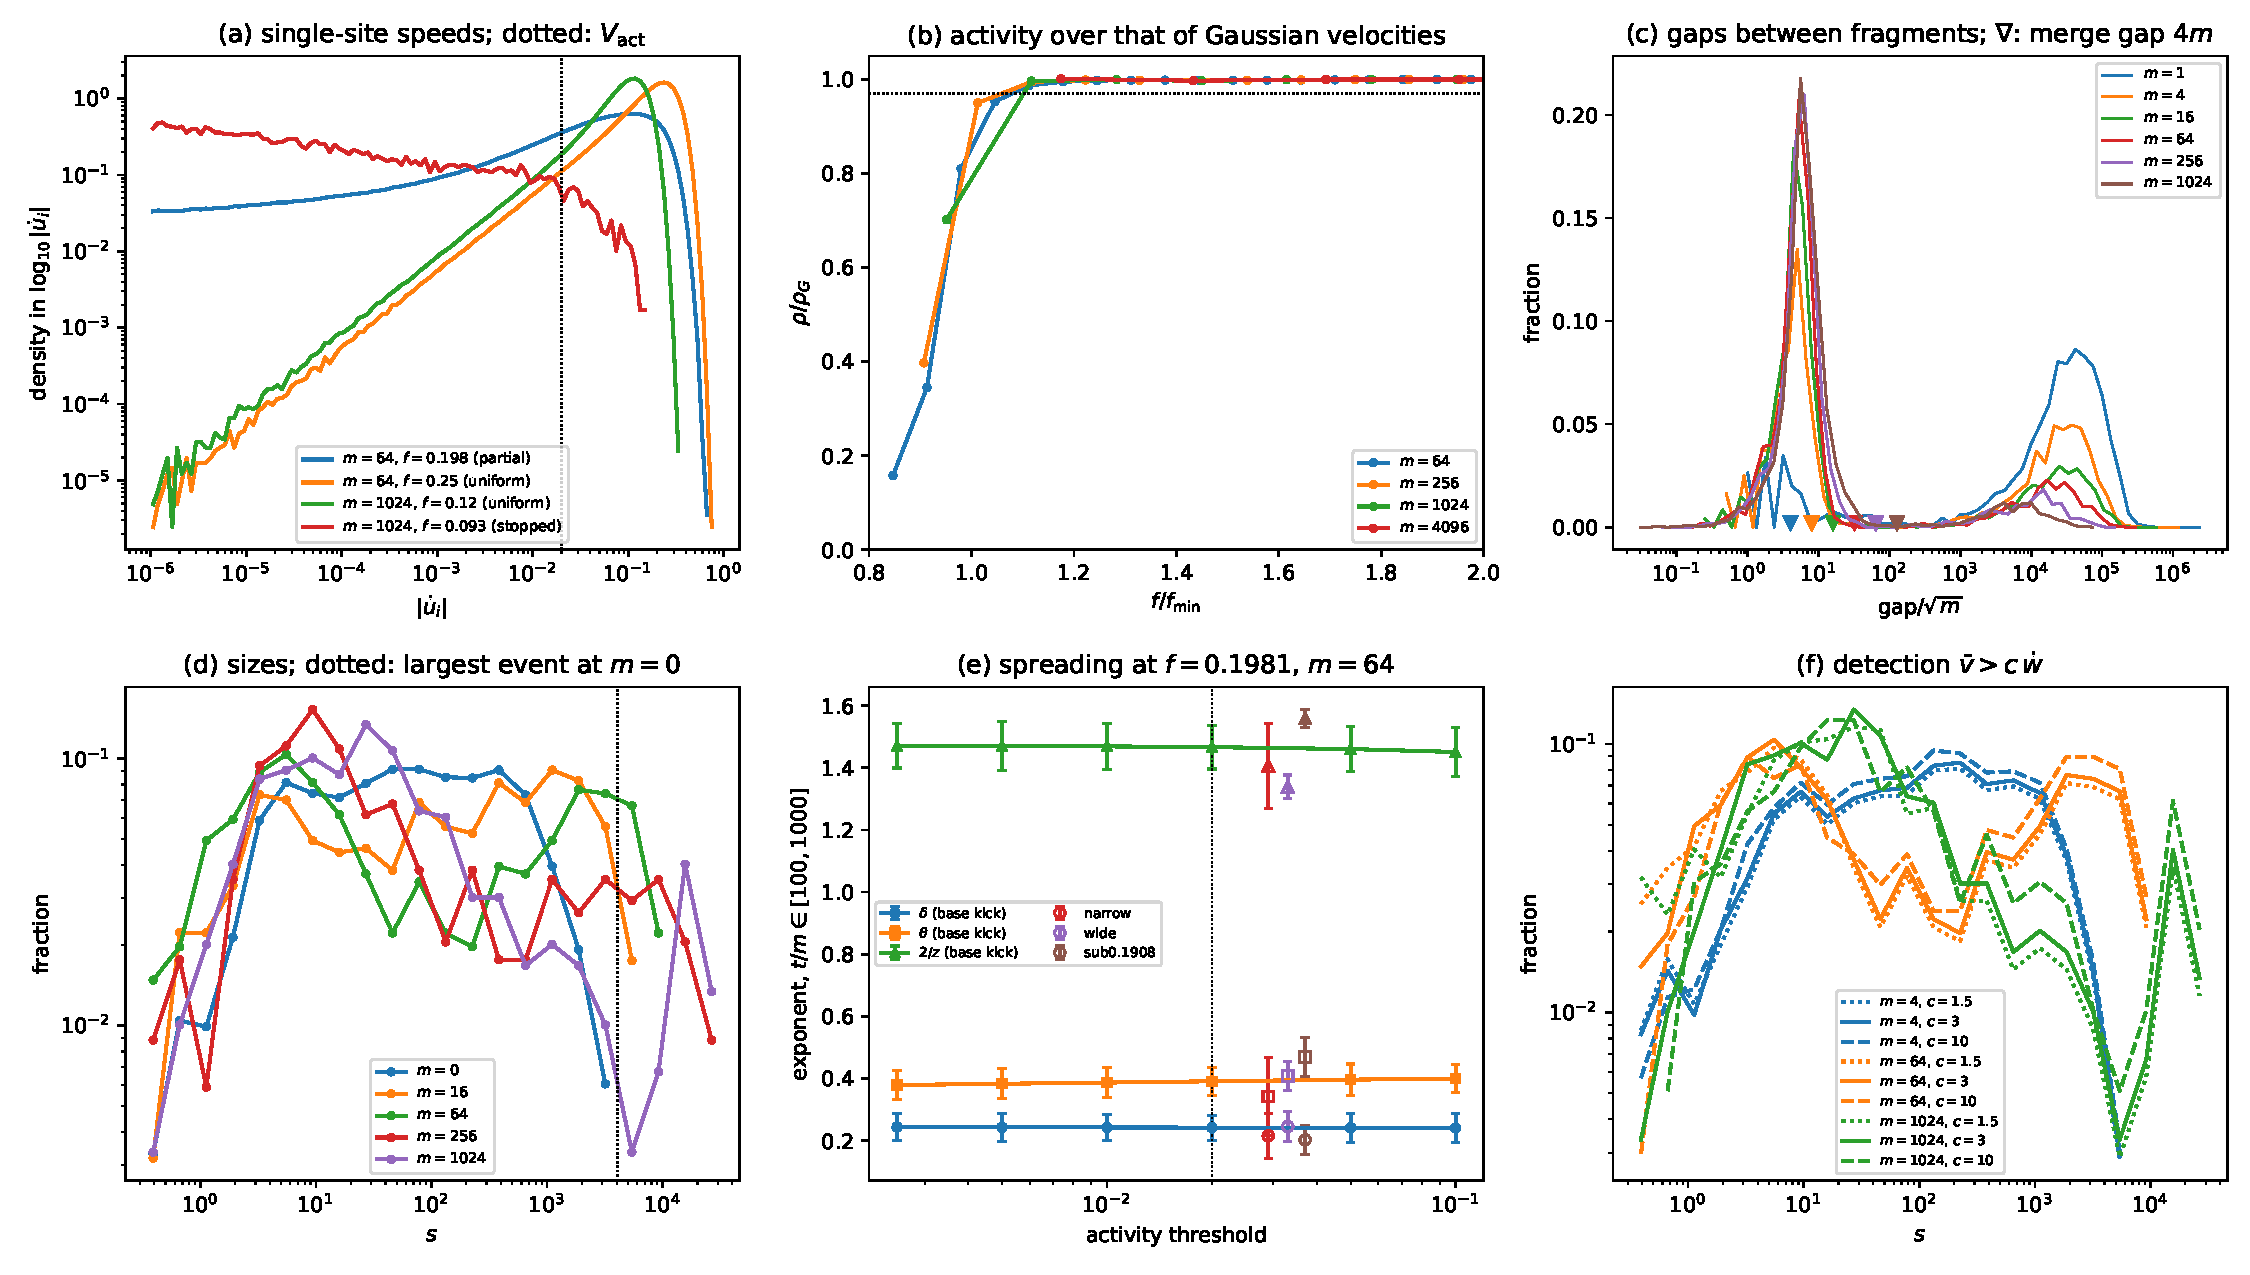
\includegraphics[width=\textwidth]{thresholds.pdf}
\caption{Where the thresholds come from. (a) Single-site speeds; dotted: $V_{\rm act}$. (b) $\rho/\rho_G$ against $f/f_{\min}$; dotted: $1-0.03$. (c) Gaps between avalanche fragments against gap$/\sqrt m$; triangles: $4m$. (d) Avalanche sizes; dotted: largest event at $m=0$. (e) Spreading exponents against the activity threshold (filled) and for other seeds and substrates (open). (f) Avalanche sizes for detection thresholds $c=1.5$, 3, 10.}
\label{fig:thresholds}
\end{figure}

%======================================================================
\section{Known results and questions}
\label{sec:known}

\begin{itemize}
\item \textbf{Overdamped line.} No-passing (Middleton 1992) gives a unique threshold $\fd=\fu=\fcs$ and a continuous transition in the qEW class: in $d=1$, $\zeta\simeq1.25$, $\beta\simeq0.25$, $\nu\simeq1.33$, $z\simeq1.43$ (Ferrero, Bustingorry, Kolton 2013). At large $\bar v$ pinning is a second-order correction (Larkin--Ovchinnikov).
\item \textbf{Inertia and overshoots.} Fisher (1998): inertia can make depinning first order. Schwarz and Fisher: overshoot automata have a mean-field tricritical point and finite-dimensional hysteresis that vanishes in large samples. de Geus and Wyart (2022, 2024): an inertial line with a non-monotonic flow curve whose minimum is measured, not computed. Amorphous solids with inertia: modified avalanche statistics. Detailed comparison in Sec.~\ref{sec:lit}.
\end{itemize}
Missing: a theory, for true inertia in a finite-dimensional line, of the sliding branch, the threshold, and their dependence on $m$ and on the disorder. Questions:
\begin{description}
\item[Q1] What sets the threshold of an inertial line, and can it be computed?
\item[Q2] Is the transition continuous or discontinuous?
\item[Q3] Is there hysteresis ($\fu\ne\fd$) in an infinite system at long times?
\item[Q4] How does the threshold scale with mass, and does the disorder class matter?
\item[Q5] Where does the crossover from qEW happen, and is it universal?
\item[Q6] What does displacement (well) driving show?
\item[Q7] What are $\zeta$ and $\tau$, and which field theory gives them?
\end{description}

%======================================================================
\section{Results at a glance}
\label{sec:glance}

\begin{center}\small
\begin{tabular}{p{0.6cm}p{11.2cm}p{2.6cm}}
\toprule
 & answer & where \\
\midrule
Q1 & $M\gtrsim5$: end of the hot branch. Closure $f_{\min}(M)$; long-time threshold $f_\infty=(0.975$--$0.99)f_{\min}$ at every mass ($0.987f_{\min}$ at $m=64$). $M\lesssim0.5$: the qEW $\fcs\simeq0.30$. & \ref{sec:closure}, \ref{sec:invasion}, \ref{sec:patchy} \\
Q2 & Uniform hot sliding ends at $f_{\min}$ with finite $v$; patchy sliding below it ends continuously at $f_\infty$, an absorbing-state transition with no rare regions. Spreading: $\delta\simeq0.2$, $\theta\simeq0.4$, and superdiffusive $z\simeq1.31\pm0.03$ (largest run), with a systematic spread $2/z=1.34$--$1.57$ between seeds and substrates: not DP ($2/z=1.265$); conserved DP ($1.40$--$1.44$) not excluded. & \ref{sec:patchy} \\
Q3 & No. Ramp hysteresis shrinks as $L^{-1/2}$; below $f_\infty$ sliding dies in a finite time. & \ref{sec:finite} \\
Q4 & $f_*\propto m^{-1/4}$ is pre-asymptotic; Debye--Waller smearing gives $f_{\min}\propto m^{-3/10}$ (RF), $m^{-5/14}$ (RB); thresholds collapse in $M$. & \ref{sec:heavy} \\
Q5 & At $M\approx0.5$ (RF), earlier for RB: overshoot of single jumps, set by the microscopic well stiffness, not universal. & \ref{sec:small} \\
Q6 & Stick--slip for $M\gtrsim6$: slips ride the hot branch, kinetic friction $\simeq f_{\min}$, onset overloaded up to $1.59f_{\min}$. & \ref{sec:aval} \\
Q7 & Cold line ($M\lesssim0.5$): qEW, $\tau=1.1\pm0.05$. Hot line: EW, $\zeta=1/2$, $T_{\rm lw}=S_\xi(0)/2\eta_{\rm eff}$, $S_\xi(0)$ from DMFT. End of sliding: absorbing-state transition with $z\simeq1.3$, not DP. & \ref{sec:dmft}, \ref{sec:rough}, \ref{sec:patchy}, \ref{sec:tau} \\
\bottomrule
\end{tabular}
\end{center}

\begin{center}\small
\begin{tabular}{p{2.3cm}p{6.2cm}p{6.6cm}}
\toprule
regime & threshold & sliding state \\
\midrule
$M\lesssim0.5$ & $\fd=\fu=\fcs$ & qEW, continuous \\
$0.5\lesssim M\lesssim5$ & lowered by overshoots of single jumps & qEW-like at small scales; under slow driving the shift grows relative to the critical window as $\xi$ grows \\
$M\gtrsim20$ & $f_\infty\simeq0.98f_{\min}$, continuous absorbing-state end of patchy sliding, $z\simeq1.3$ & hot radiating string, $T_{\rm kin}\simeq\langle F^2\rangle\sqrt{m/\kappa}/2\eta$; EW at large scales \\
$M\gg1$ & $f_{\min}\propto m^{-3/10}$ (RF), $m^{-5/14}$ (RB) & $T\propto m^{2/(4+a)}$ \\
\bottomrule
\end{tabular}
\end{center}

%======================================================================
\section{Exact relations}
\label{sec:exact}

\paragraph{Thresholds.} Equilibria solve $\kappa\Delta u+F(u)+f=0$, independent of $m$ and $\eta$, so $\fcs$ does not depend on $m$. Nothing stops above $\fcs$, and a line that starts at $\fu$ keeps sliding there, so $\fd\le\fu\le\fcs$. At $m=0$ no-passing makes them equal; for $m>0$ it fails.

\paragraph{Power balance.} In a steady sliding state the work of the disorder grows only like $\sqrt{\bar vt}$, so $f\bar v=\eta\langle\dot u^2\rangle$:
\begin{equation}
\boxed{\;f-\eta\bar v=\frac{\eta\langle\delta\dot u^2\rangle}{\bar v}\;},\qquad T_{\rm kin}=\frac{m\bar v(f-\eta\bar v)}{\eta}.
\label{eq:identity}
\end{equation}
The simulations satisfy it to $0.1\%$ on average.

\paragraph{MSRJD action.} Averaging over the disorder gives
\begin{equation}
\mathcal S[u,\hat u]=\int_{x,t}\hat u\big(m\ddot u+\eta\dot u-\kappa\nabla^2u-f\big)-\frac12\int_x\!\int_{t,t'}\hat u_{x,t}\hat u_{x,t'}\,\Delta(u_{x,t}-u_{x,t'}),
\label{eq:msr}
\end{equation}
with bare response $R_q(\omega)=1/(\lambda_q-m\omega^2-i\eta\omega)$, $\lambda_q=2\kappa(1-\cos q)$. The disorder vertex is \emph{local in $x$}. Every theory below is an expansion of Eq.~\eqref{eq:msr} around a different state:
\begin{itemize}
\item around the cold static fixed point: functional RG (Sec.~\ref{sec:small});
\item around uniform sliding at velocity $\bar v$: second order, the closure, and the single-site DMFT (Sec.~\ref{sec:hot});
\item around coexisting hot and pinned regions: no expansion in $\Delta$ works; the coarse-grained activity obeys Reggeon field theory (Sec.~\ref{sec:patchy}).
\end{itemize}

%======================================================================
\section{The hot sliding state}
\label{sec:hot}

\subsection{Second order: friction is radiation}
\label{sec:second}

Write $u_i=\bar vt+\delta u_i$. To lowest order site $i$ is driven by $F_i(\bar vt)$, spectrum $\hat\Delta(\omega/\bar v)/\bar v$, and only the local susceptibility enters:
\begin{gather}
\chi(\omega)=\int\frac{dq}{2\pi}\frac{1}{\lambda_q-m\omega^2-i\eta\omega}=\frac{1}{\sqrt{z(z-4\kappa)}},\qquad z=m\omega^2+i\eta\omega,\nonumber\\
f(\bar v)=\eta\bar v+\frac{P(\bar v)}{\bar v},\qquad P=\int_0^\infty\frac{d\omega}{\pi}S(\omega)\,\omega\,\mathrm{Im}\chi .
\label{eq:flow2}
\end{gather}
\begin{itemize}
\item \textbf{Radiation.} For $\eta/m\ll\omega<2\sqrt{\kappa/m}$, $\omega\,\mathrm{Im}\chi\to1/2\sqrt{\kappa m}$: a string point is a dashpot of twice the string impedance $Z=\sqrt{\kappa m}$, and energy leaves as sound. Then
\begin{equation}
P_{\rm rad}=\frac{\langle F^2\rangle}{2\sqrt{\kappa m}},\qquad T_{\rm kin}=\frac{\langle F^2\rangle}{2\eta}\sqrt{\frac{m}{\kappa}},
\end{equation}
independent of $\bar v$ and $\eta$. The line is hot: $T_{\rm kin}\approx3.6$ at $m=1024$, against site barriers $\sim Ar_f/2$.
\item \textbf{Minimum.} $f=\eta\bar v+P_{\rm rad}/\bar v$ has a minimum $f_*=(2\eta\langle F^2\rangle/\sqrt{\kappa m})^{1/2}$ at $v_*=(\langle F^2\rangle/2\eta\sqrt{\kappa m})^{1/2}$ ($f_*/\fcs\sim M^{-1/4}$). Second order fails exactly there ($\langle\delta u^2\rangle\sim(v_*/\bar v)^2r_f^2$), so $f_*$ is a scale, not a prediction.
\item \textbf{Test} (Fig.~\ref{fig:flow}; $L=4096$, 4 samples). For $m\le1$ the flow curve is the qEW one, ending at $\fcs\simeq0.30$. With mass the sliding branch extends far below $\fcs$ (to $0.06$ at $m=4096$). Second order is accurate for $\bar v>0.25$ (within 10\%).
\end{itemize}

\begin{figure}[H]
\centering
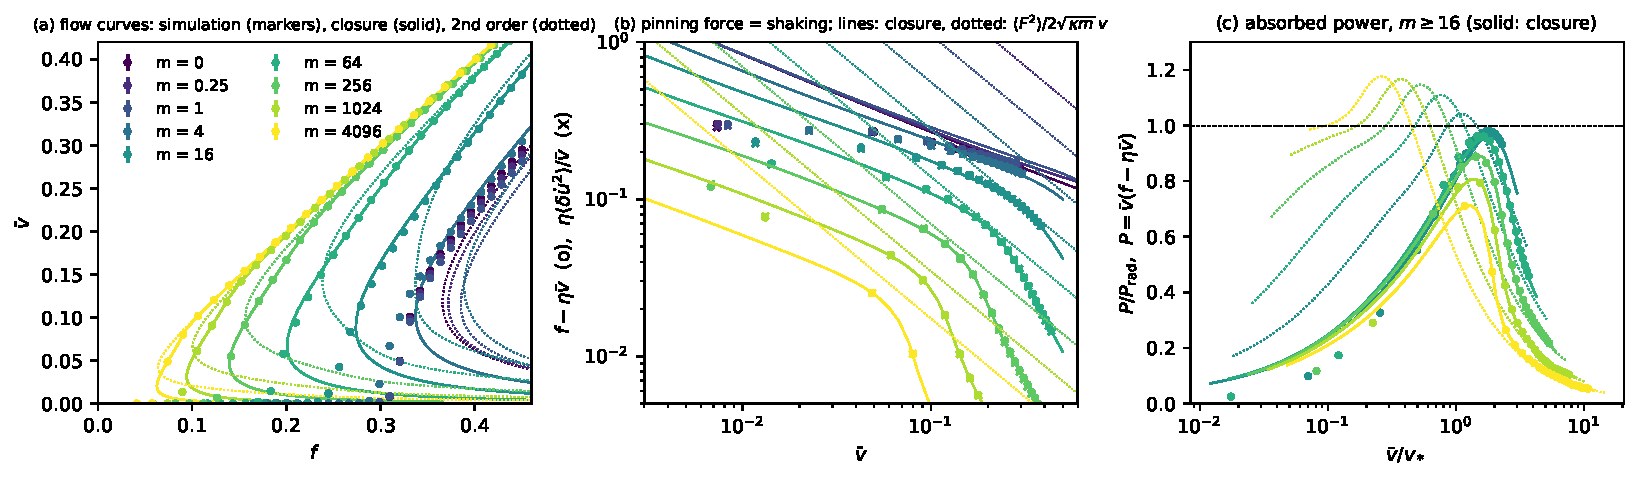
\includegraphics[width=\textwidth]{flow_curves.pdf}
\caption{(a) Flow curves, $L=4096$: simulation (markers), closure (solid), second order (dotted). (b) Both sides of Eq.~\eqref{eq:identity}: $f-\eta\bar v$ (circles) and $\eta\langle\delta\dot u^2\rangle/\bar v$ (crosses); dotted: $P_{\rm rad}/\bar v$. (c) Absorbed power over $P_{\rm rad}$ against $\bar v/v_*$, $m\ge16$.}
\label{fig:flow}
\end{figure}

\subsection{Hot-line closure: $f_{\min}$}
\label{sec:closure}

\paragraph{Definition.} Dress the second-order pinning force by Gaussian displacement fluctuations of an equilibrium string at temperature $T$, $B_T(\tau)=T\,b(\tau)$, $b(\tau)=2\int\frac{dq}{2\pi}\frac{1-c_q(\tau)}{\lambda_q}$:
\begin{equation}
F_{\rm pin}(v,T)=-\int_0^\infty d\tau\,R(\tau)\,\Delta'_{Tb(\tau)}(v\tau),
\label{eq:Fpin}
\end{equation}
$\Delta_s$ the correlator smeared by a Gaussian of variance $s$, and fix $T$ by the exact power balance, $T=mvF_{\rm pin}(v,T)/\eta$. Then $f(v)=\eta v+F_{\rm pin}(v,T(v))$ and $f_{\min}(M)$ is its minimum. No free parameter (\texttt{src/sc.py}).

\paragraph{Results.} $f_{\min}=c\,f_*$ with $c=0.82$, $0.85$, $0.84$, $0.80$, $0.75$ for $m=16$ to 4096. For $m\lesssim10$, $f_{\min}>\fcs$: the hot branch is preempted by ordinary depinning. The closure follows the measured flow curves to three decimals in $\bar v$ for $m\ge64$ and to $\lesssim10\%$ at $m=4$--16.

\paragraph{Right for the right reason?} For uniformly sliding lines at $m=64$--4096 (\texttt{runs/check\_closure.py}; Fig.~\ref{fig:edges}a,b): $T_{\rm kin}$ agrees to 1--3\%, $F_{\rm pin}$ to 2--3\%, and increments are nearly Gaussian (excess kurtosis $\le0.25$). But $B$ has the wrong shape: $B/Tb\approx0.65$ at short lags and $1.4$--$2.6$ at long lags, because the driven noise is coloured. The agreement partly comes from compensating errors, so closure numbers carry a $\sim10\%$ systematic. Variants that fix the shape (\texttt{archive/sc\_noneq.py}, \texttt{archive/sc\_hybrid.py}) fit $B$ better but lose the sharp minimum. The closure stays the best threshold predictor: $f_\infty$ lies 1--2.5\% below its $f_{\min}$. Section~\ref{sec:dmft} replaces it for the noise.

\subsection{Single-site (DMFT) theory}
\label{sec:dmft}

Because the vertex in Eq.~\eqref{eq:msr} is local, one site can be solved exactly in a Gaussian bath formed by the rest of the line (dynamical cavity, DMFT). It becomes exact for many neighbours; for the chain it is uncontrolled, and it cannot describe coexistence, because the bath is uniformly hot by construction.

\paragraph{Bath.} Model the other sites as a linear medium: friction $\eta_{\rm eff}$, independent Gaussian force noises of spectrum $S_\xi(\omega)$, drift $\bar v$. Integrating out the two half-chains gives site 0 the equation
\begin{equation}
m\ddot w_0+\eta\dot w_0+\int K(t-s)\,w_0(s)\,ds=F_0(\bar vt+w_0)+(f-\eta\bar v)+\zeta(t),\qquad
K(\omega)=\sqrt{a(a+4\kappa)}-a,
\end{equation}
$a(\omega)=-m\omega^2-i\eta_{\rm eff}\omega$, with $K\propto\sqrt{-i\omega}$ at small $\omega$ (the semi-infinite string), and Gaussian cavity noise $S_\zeta=2\kappa^2S_\xi|G|^2/(1-\kappa^2|G|^2)$, $G=(2\kappa-K)/2\kappa^2$. Self-consistency: $S_\xi$ is the spectrum of the force $F_0$ that site 0 itself feels; $\eta_{\rm eff}=\partial f/\partial\bar v$ at fixed bath; $f(\bar v)=\eta\bar v-\langle F_0\rangle$.

\paragraph{Two solutions.}
\begin{itemize}
\item \textbf{Numerical cavity} (\texttt{src/cavity.py}). Site 0 in its real landscape is embedded in a ring of 63--127 linear medium sites with coloured noise; $S_\xi$ and $\eta_{\rm eff}$ are iterated to a fixed point (6 passes, then a polish with 32 rings).
\item \textbf{Gaussian DMFT} (\texttt{src/gdmft2.py}). The cavity's force correlator is the disorder correlator smeared by the true displacement spread, so keep only that. Linearising the mean force in the site's own past displacement, $\delta\langle F(t)\rangle=\int ds\,R(t-s)\langle\Delta''(u_t-u_s)\rangle[\delta u(t)-\delta u(s)]$, gives the disorder self-energy, and the theory closes on deterministic maps whose only inputs are $m,\kappa,\eta,\Delta,\bar v$:
\begin{align}
C(t)&=\big\langle\Delta(\bar vt+x)\big\rangle_{x\sim\mathcal N(0,B(t))}, &
S_\xi(\omega)&=2\!\int_0^\infty\!C(t)\cos\omega t\,dt,\nonumber\\
\Sigma(\omega)&=\int_0^\infty\!dt\,R_{\rm loc}(t)\big\langle\Delta''(\bar vt+x)\big\rangle\,(1-e^{i\omega t}), &
z(\omega)&=m\omega^2+i\eta\omega+\Sigma(\omega),\nonumber\\
B(t)&=\frac2\pi\int_0^\infty\!d\omega\,S_\xi(\omega)\frac{\mathrm{Im}\,g(z)}{\mathrm{Im}\,z}(1-\cos\omega t), &
R_{\rm loc}(t)&=\frac2\pi\int_0^\infty\!d\omega\,\mathrm{Im}\,g(z)\sin\omega t,
\label{eq:gdmft}
\end{align}
with $g(z)=1/\sqrt{z(z-4\kappa)}$ (the chain's local propagator; no fluctuation--dissipation assumption), $\langle F\rangle=\int R_{\rm loc}\langle\Delta'\rangle dt$, $f=\eta\bar v-\langle F\rangle$. $\Sigma(0)=0$: the disorder exerts no static restoring force. Its slope gives the zero-frequency friction $\eta_{\rm eff}=\eta-\int t\,R_{\rm loc}\langle\Delta''\rangle dt$, and $T_{\rm lw}=S_\xi(0)/2\eta_{\rm eff}$. Above $\omega\sim\bar v$, $\Sigma$ decays and the friction returns to $\eta$. The fixed point takes 10--60 iterations of under a second.
\item \textbf{Why $\Sigma(\omega)$.} A first version (\texttt{src/gdmft.py}) damped the medium with the constant $\eta_{\rm eff}\approx0.6$ at all frequencies. Its high-frequency fluctuations were then too large: $T_{\rm kin}$ exceeded the exact power balance, Eq.~\eqref{eq:identity}, by 18--32\%. With $\Sigma(\omega)$, which comes from the same one-loop action as the noise, the approximation conserves energy: Eq.~\eqref{eq:identity} holds to better than 1\% at every point computed, for all three masses.
\end{itemize}

\paragraph{Results} at the four points where $C(t)$ and $B(t)$ were measured (\texttt{runs/sq\_diag.py}; Fig.~\ref{fig:dmft}; entries simulation / numerical cavity / Gaussian DMFT with $\Sigma(\omega)$):

\begin{center}\footnotesize\setlength{\tabcolsep}{4pt}
\begin{tabular}{lccccc}
\toprule
$m$, $f$ ($\bar v$) & $S_\xi(0)$ [bare $\hat\Delta(0)/\bar v$] & $f(\bar v)$ & $\eta_{\rm eff}$ & $T_{\rm lw}$ & $T_{\rm kin}$ \\
\midrule
1024, 0.12 (0.089) & 6.03 / 5.94 / 6.07 [3.74] & 0.120 / 0.122 / 0.121 & 0.60 / 0.53 / 0.57 & 5.0 / 5.6 / 5.3 & 2.82 / 2.86 / 2.91 \\
1024, 0.11 (0.071) & 8.71 / 9.24 / 8.71 [4.71] & 0.110 / 0.110 / 0.111 & 0.67 / 0.70 / 0.62 & 6.5 / 6.6 / 7.0 & 2.83 / 3.19 / 2.89 \\
1024, 0.10 (0.051) & 13.8 / 14.3 / 13.4 [6.51] & 0.100 / 0.091 / 0.100 & 0.63 / 0.90 / 0.79 & 10.9 / 7.9 / 8.5 & 2.55 / 3.46 / 2.55 \\
256, 0.17 (0.117) & 4.47 / 4.81 / 4.73 [2.85] & 0.170 / 0.169 / 0.171 & 0.61 / 0.67 / 0.62 & 3.7 / 3.6 / 3.8 & 1.59 / 1.95 / 1.63 \\
\bottomrule
\end{tabular}
\end{center}
\begin{itemize}
\item \textbf{Noise.} $S_\xi(0)$, 1.6--2.1 times the bare value, is predicted within 1--6\%, and $C(t)$ is reproduced at all lags (rms error $5\times10^{-4}$ against $C(0)=0.22$). The Gaussian DMFT also reproduces $B(t)$ out to $t=3000$, including the EW tail; the finite cavity ring cuts it off beyond $t\approx300$.
\item \textbf{Force and temperature.} With $\Sigma(\omega)$ the flow curve is within 1\% and $T_{\rm kin}$ within 3\% at all four points, including the one next to $f_{\min}$. $T_{\rm lw}$ is within 3--7\% at the three faster points and 22\% low at $\bar v=0.051$, where $\eta_{\rm eff}$ comes out $0.79$ against $0.63$.
\item \textbf{Why the noise is enhanced: local time.} If the spread is wider than a disorder cell, $S_\xi(0)\approx\hat\Delta(0)\,\ell$ with $\ell=2\int_0^\infty dt\,e^{-\bar v^2t^2/2B}/\sqrt{2\pi B}$, the mean time a site spends near a point of its own trajectory (bare: $1/\bar v$). For $B\propto t^{2H}$ this gives exactly $S_\xi(0)=\hat\Delta(0)/[(1-H)\bar v]$, independent of temperature: $4/3$ for EW wandering ($H=1/4$), $2$ for diffusive ($H=1/2$), log-divergent for ballistic. Here the spread is only about one cell at the crossing, so this estimate is 30--40\% high and the full smearing of Eq.~\eqref{eq:gdmft} is needed.
\item \textbf{The uniform branch does not end at $f_\infty$} (\texttt{runs/dmft\_flow.py}; Fig.~\ref{fig:dmftflow}). Down to the lowest measured uniform sliding states the theory follows the simulated flow curves at $m=64$, 256 and 1024. Below them it keeps a stable hot solution ($\eta_{\rm eff}>0$, $\mathrm{Im}\,z>0$ at all $\omega$) to well below where the real line stops. At $m=1024$ it has a shallow minimum, $0.087$ at $\bar v\approx0.015$, 5\% below $f_\infty\approx0.092$; at $m=256$ and 64, $f$ keeps falling to $0.111$ and $0.128$ at $\bar v=0.006$--$0.01$, against $f_\infty\approx0.137$ and $0.198$. So the end of sliding is not a spinodal of uniform sliding: it is the nucleation of pinned patches, which a local theory with a uniformly moving bath cannot describe. At such low $\bar v$ the line is also no longer hot ($T_{\rm kin}=0.08$ at $m=64$, $\bar v=0.01$, against barriers $\sim0.5$), so the Gaussian displacements assumed in the smearing fail. The closure's minimum lies within 1--2.5\% of $f_\infty$, but its back-bending comes from an equilibrium-shaped $B$ that the measurements contradict (Sec.~\ref{sec:closure}).
\end{itemize}
\begin{figure}[H]
\centering
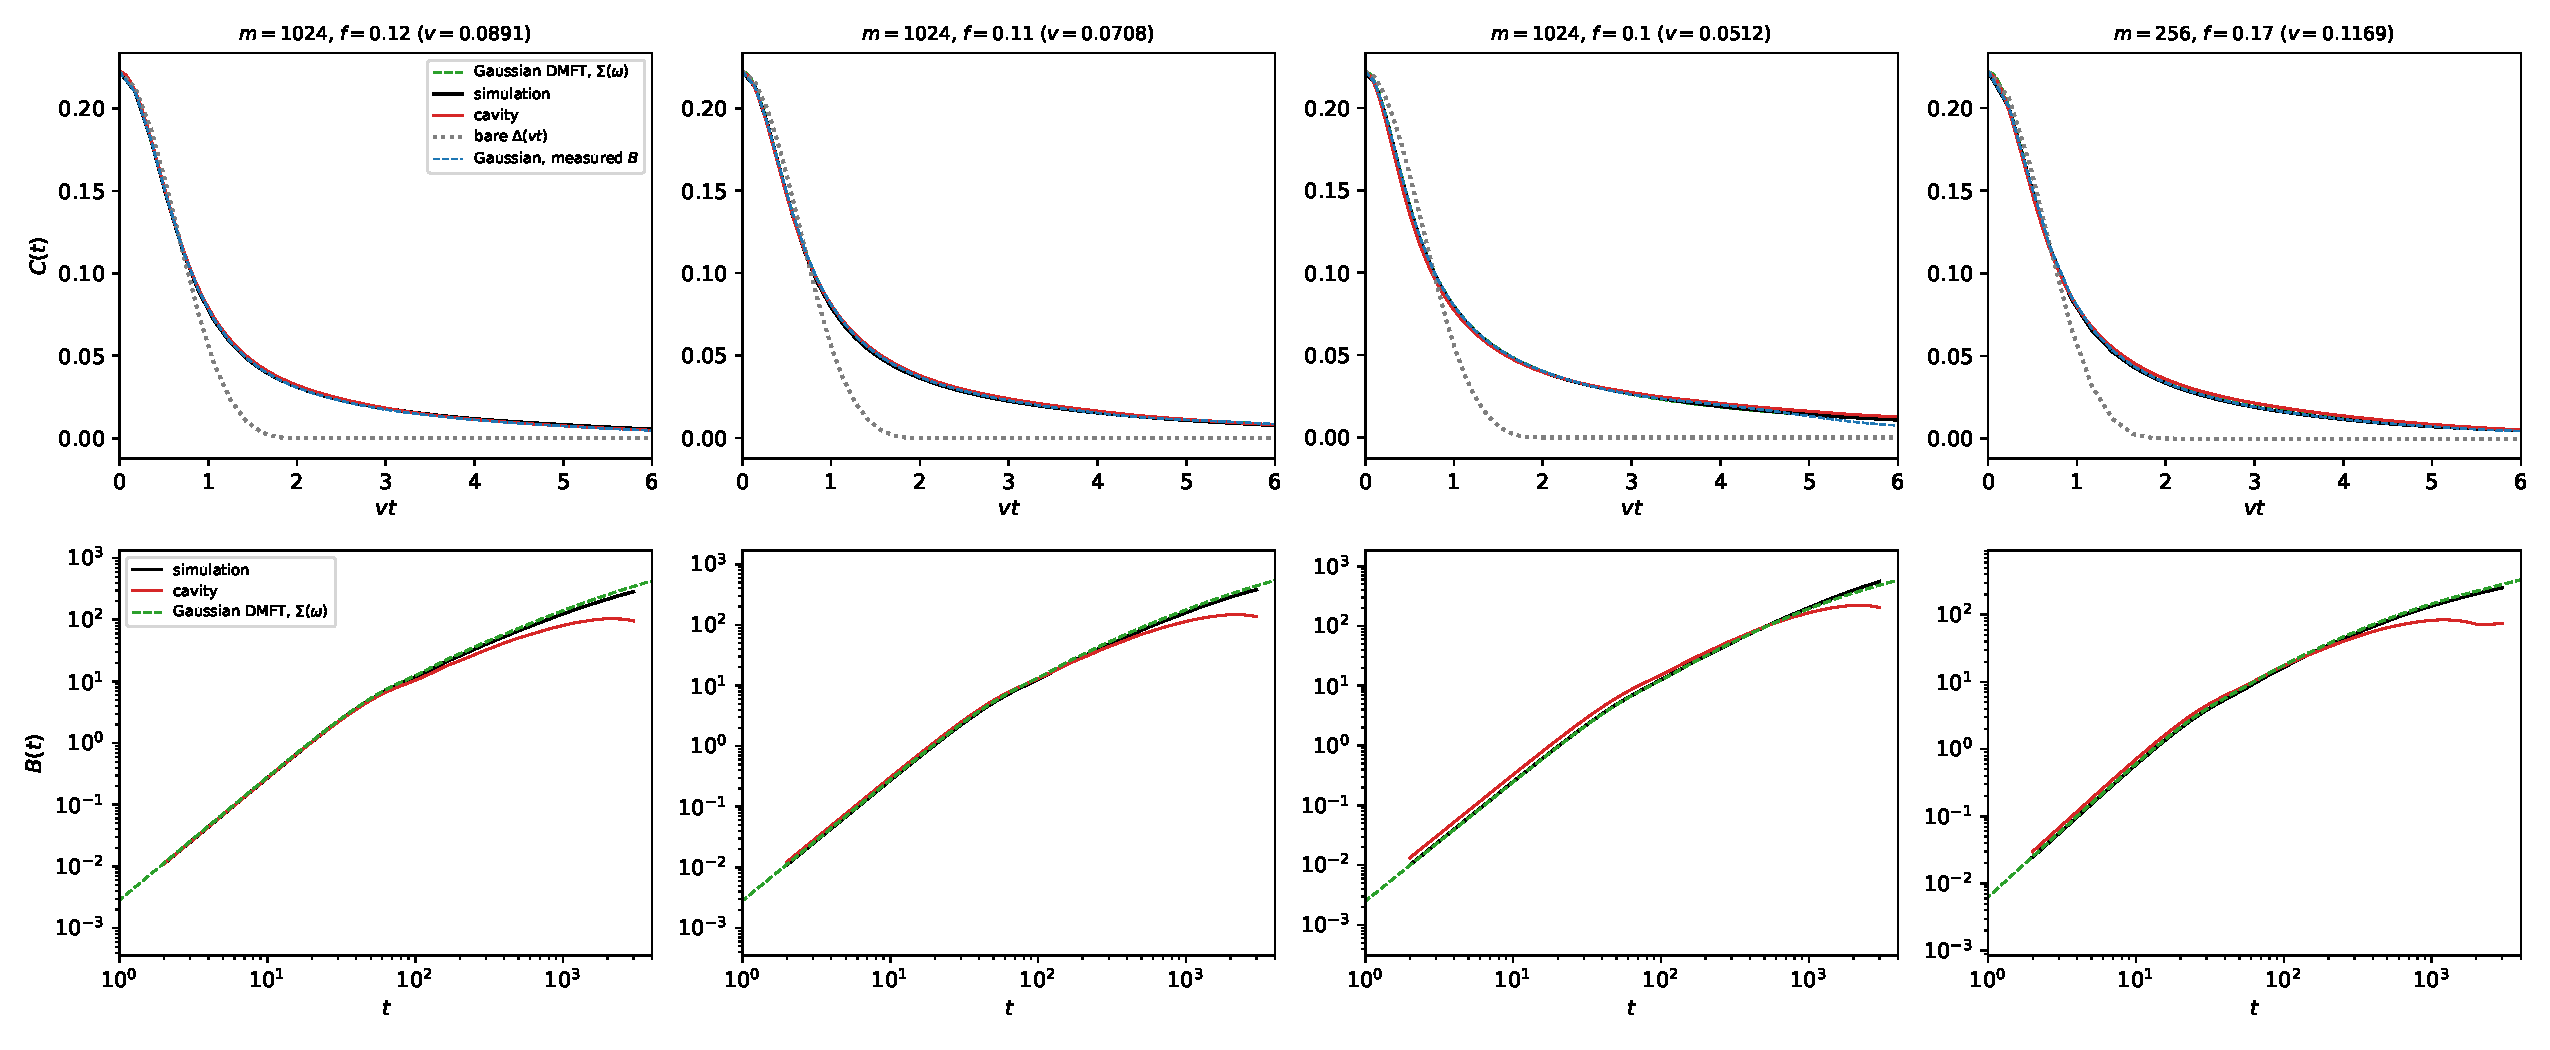
\includegraphics[width=\textwidth]{single_site.pdf}
\caption{Single-site theory against the simulated hot line. Top: force autocorrelation $C(t)$ against $\bar vt$: simulation, numerical cavity, Gaussian DMFT, bare $\Delta(\bar vt)$, and Gaussian smearing with the measured $B$. Bottom: displacement spread $B(t)$ (relative to the line mean); the cavity ring (64 sites) saturates beyond $t\approx300$, and the dip near $t\approx2000$ is sound circling the ring.}
\label{fig:dmft}
\end{figure}

\begin{figure}[H]
\centering
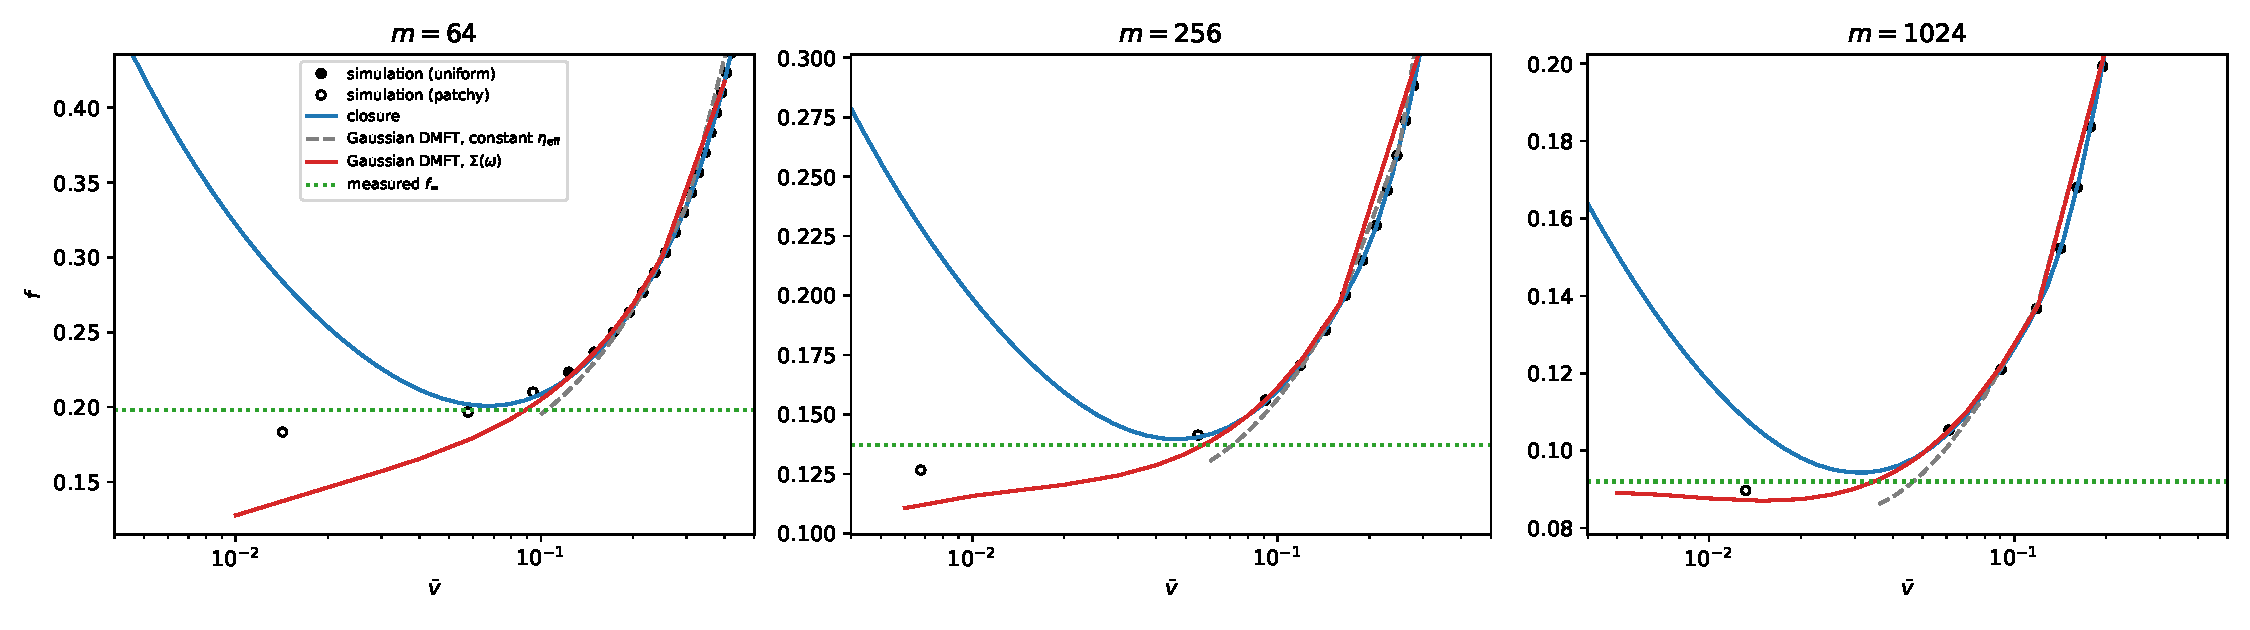
\includegraphics[width=\textwidth]{dmft_flow.pdf}
\caption{Flow curves: simulation ($L=4096$; filled: uniform sliding, open: patchy, finite time), closure, Gaussian DMFT with constant $\eta_{\rm eff}$ (dashed) and with $\Sigma(\omega)$ (red), and the measured long-time threshold $f_\infty$ (dotted).}
\label{fig:dmftflow}
\end{figure}

\subsection{Roughness and scale-dependent temperature}
\label{sec:rough}

At large scales the moving line sees the disorder as noise varying in time. Statistical tilt symmetry forbids a KPZ term, so the line is Edwards--Wilkinson. Mode $q$ is driven by the single-site noise and damped by $\eta_{\rm eff}$:
\begin{equation}
S(q)=\int\frac{d\omega}{2\pi}\frac{S_\xi(\omega)}{|\lambda_q-m\omega^2-i\eta_{\rm eff}\omega|^2},\qquad
T_{\rm lw}\equiv\lim_{q\to0}\lambda_qS(q)=\frac{S_\xi(0)}{2\eta_{\rm eff}}.
\label{eq:Tlw}
\end{equation}
Underdamped modes feel the noise at their own frequency, $T(q)\approx S_\xi(\omega_q)/2\eta$; slow modes feel $S_\xi(0)$. At second order $S_\xi(0)=\hat\Delta(0)/\bar v$, $\eta_{\rm eff}=\eta$, so $T_{\rm lw}=A^2/6\eta\bar v$ (RF) and $0$ (RB).

Measured at $L=2048$ (8 samples; \texttt{runs/sq.py}, \texttt{runs/sq\_near.py}, \texttt{runs/sq\_diag.py}; Fig.~\ref{fig:rough}):
\begin{itemize}
\item \textbf{$\zeta=1/2$.} $\lambda_qS(q)$ is flat over two decades at small $q$, and each mode is in equipartition, $\lambda_qS(q)\simeq m\langle|\dot u_q|^2\rangle/L$, at a temperature that depends on scale: at $m=1024$, $f=0.12$, $T_{\rm lw}=5.0$, $1.9$ at the lattice scale, $T_{\rm kin}=2.8$.
\item \textbf{Random bond.} $T_{\rm lw}$ is suppressed fifty-fold ($0.01$ against $0.5$ at the lattice scale), as $\hat\Delta(0)=0$ predicts.
\item \textbf{Large-scale temperature.} Bare second order is 2.6--3.3 times too low. Measured: $T_{\rm lw}=10.9$, $6.5$, $5.0$ ($m=1024$, $f=0.10$, $0.11$, $0.12$), $3.7$ ($m=256$, $f=0.17$). Eq.~\eqref{eq:Tlw} with the measured $S_\xi(0)$ and the closure's differential friction $\eta+\partial_vF_{\rm pin}|_T$ ($0.56$--$0.65$) gives $10.6$, $7.3$, $5.4$, $3.7$. The DMFT of Sec.~\ref{sec:dmft} predicts $S_\xi(0)$ itself. Approaching $f_{\min}$, $T_{\rm lw}$ grows through the noise, $S_\xi(0)\propto\bar v^{-1.3}$, not through $\eta_{\rm eff}\to0$.
\end{itemize}

\begin{figure}[H]
\centering
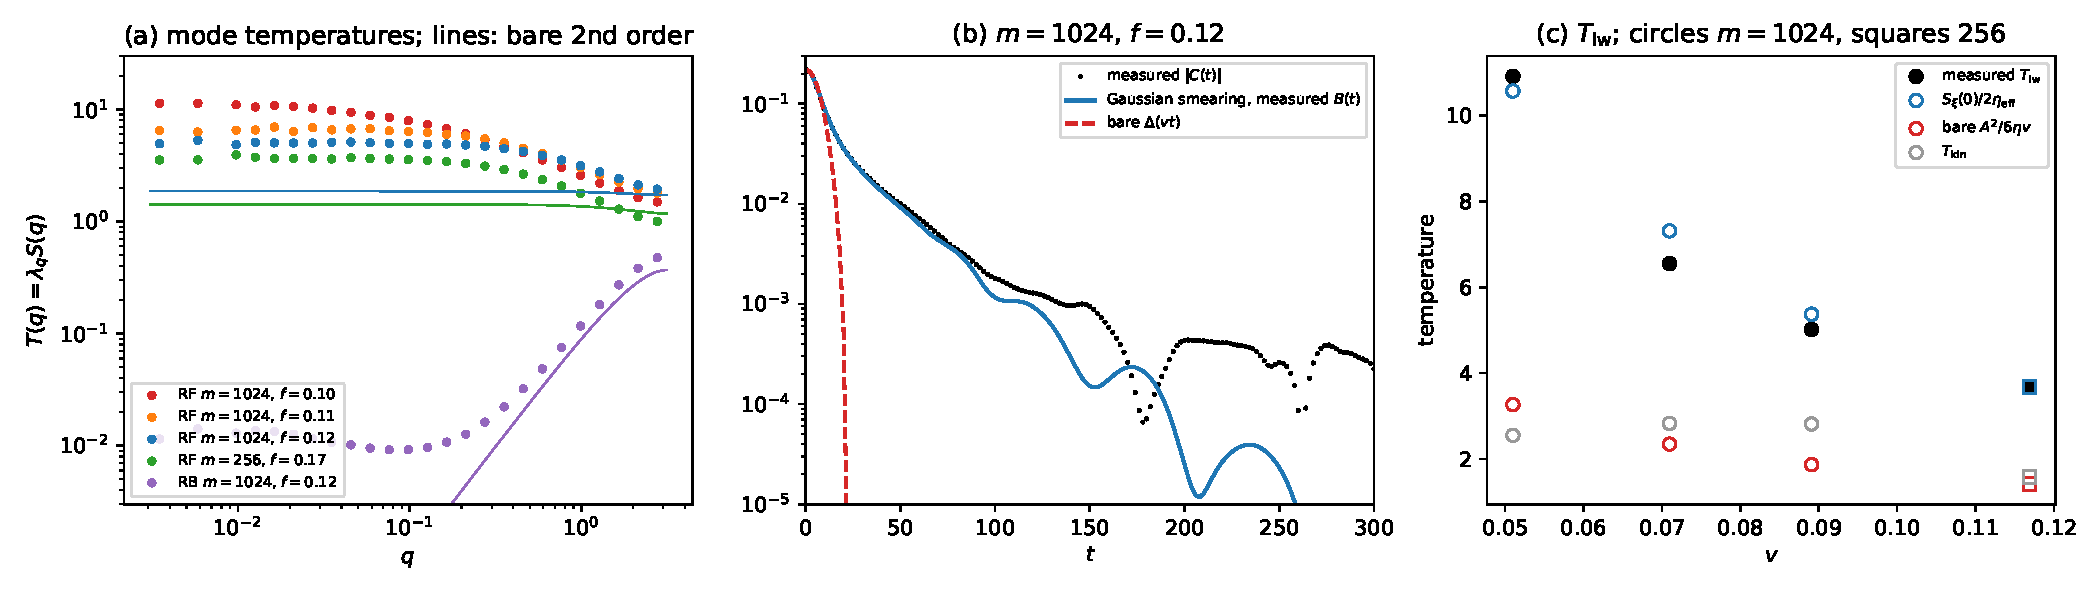
\includegraphics[width=\textwidth]{roughness.pdf}
\caption{Hot sliding line. (a) Mode temperatures $\lambda_qS(q)$; lines: bare second order. (b) $C(t)$ at $m=1024$, $f=0.12$: measured, Gaussian smearing with measured $B(t)$, bare. (c) $T_{\rm lw}$ against $\bar v$: measured, Eq.~\eqref{eq:Tlw}, bare $A^2/6\eta\bar v$, and $T_{\rm kin}$.}
\label{fig:rough}
\end{figure}

\subsection{Heavy lines and random-bond disorder}
\label{sec:heavy}

\paragraph{Theory: Debye--Waller smearing.} A hot line smears the disorder it sees. In the radiation regime $P\simeq(2Z)^{-1}\int\frac{dk}{\pi}\hat\Delta(k)e^{-k^2B/2}$, so only $k\lesssim B^{-1/2}$ contributes; with $\hat\Delta\propto k^{2n}$, $P\propto B^{-a/2}/Z$, $a=1+2n$ ($a=1$ RF, $3$ RB). With $B\simeq T(r_f/v)/Z$, $T=mP/\eta$ and $v\simeq(P/\eta)^{1/2}$:
\begin{equation}
f_{\min}\propto m^{-\frac{2+a}{2(4+a)}},\quad T\propto m^{\frac{2}{4+a}}:\qquad f_{\min}\propto m^{-3/10}\ \text{(RF)},\quad m^{-5/14}\ \text{(RB)},
\end{equation}
reducing to $m^{-1/4}$ without smearing.

\paragraph{Test} (Fig.~\ref{fig:heavy}). Closure: local slopes $-0.30$, $-0.31$ (RF, $m=4096\to65536$), $-0.33$ (RB); $T\propto m^{0.43}$. Simulations, $\fd$ at $L=1024$: $0.054$, $0.034$, $0.021$ for $m=4096$, 16384, 65536 (slopes $-0.32$, $-0.35$); RB $-0.35$. RB thresholds follow the RB closure ($\fd/f_{\min}=0.99$--$0.90$). Lifetimes at $m=16384$ confirm the closure threshold directly (Fig.~\ref{fig:gap}c).

\begin{figure}[H]
\centering
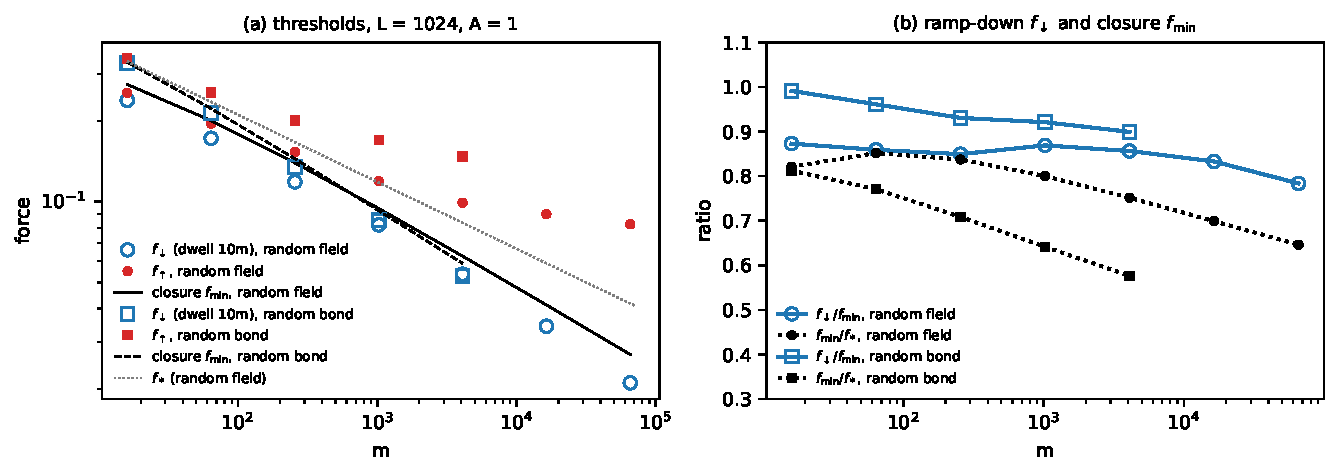
\includegraphics[width=0.85\textwidth]{large_mass_rb.pdf}
\caption{(a) Finite-time thresholds at $L=1024$, RF (circles, to $m=65536$) and RB (squares), with closure $f_{\min}$ (solid RF, dashed RB). (b) $\fd/f_{\min}$ (open) and $f_{\min}/f_*$ (dotted).}
\label{fig:heavy}
\end{figure}

%======================================================================
\section{The threshold of a heavy line}
\label{sec:threshold}

\subsection{Mechanism: hot regions invade pinned ones}
\label{sec:invasion}

A sliding domain loads its pinned neighbours with an elastic force that grows without bound, so a pinned line cannot stop a self-sustaining hot domain. Hot regions invade wherever the hot state exists and retreat where it does not. The threshold is the force $f_0$ where the edge speed $s(f)$ vanishes, near $f_{\min}$, and a domain of size $\ell_0$ below it dies in $\tau\simeq\ell_0/|s|\propto(f_0-f)^{-1}$. Unlike a bistable system with a Maxwell point, the pinned state offers essentially no resistance.

\begin{itemize}
\item \textbf{Domains.} Just below $f_{\min}$, domains of a few hundred sites slide through a pinned line, with edges at up to the sound speed (Fig.~\ref{fig:coex}).
\item \textbf{Lifetimes} (quench a sliding line, up to $200m$, 16 samples; Fig.~\ref{fig:life}). At $m=1024$ every line stops below $0.092$; the median lifetime grows from $15m$ to $155m$ for $f=0.072$ to $0.092$, as $(f_{\min}-f)^{-1.0}$ ($-1.2$ at $m=256$), nearly independent of $L$. Above $f_{\min}$ every line slides, at $\bar v=0.033$--$0.047$ (closure $v_{\min}=0.030$).
\item \textbf{Edge speed} (half hot, half pinned, $L=8192$; \texttt{runs/edges.py}; Fig.~\ref{fig:edges}c). Zero at $f_0=0.975f_{\min}$ ($m=1024$) and $0.981f_{\min}$ ($m=256$), roughly linear through zero, saturating at $0.84$--$0.93\,c$ above $1.1f_{\min}$; far below $f_{\min}$ the hot region cools in bulk instead of retreating. Lifetimes then give $\ell_0\approx800$ sites at $m=1024$.
\item \textbf{Long runs} (Fig.~\ref{fig:gap}). $m=256$, $1000m$: all lines stop at $0.974f_{\min}$, 88\% slide at $0.989f_{\min}$. $m=16384$, $200m$: all stop at $0.97f_{\min}$, all slide at $1.02f_{\min}$. At $m=64$ short runs mislead; Sec.~\ref{sec:patchy}.
\end{itemize}

\begin{figure}[H]
\centering
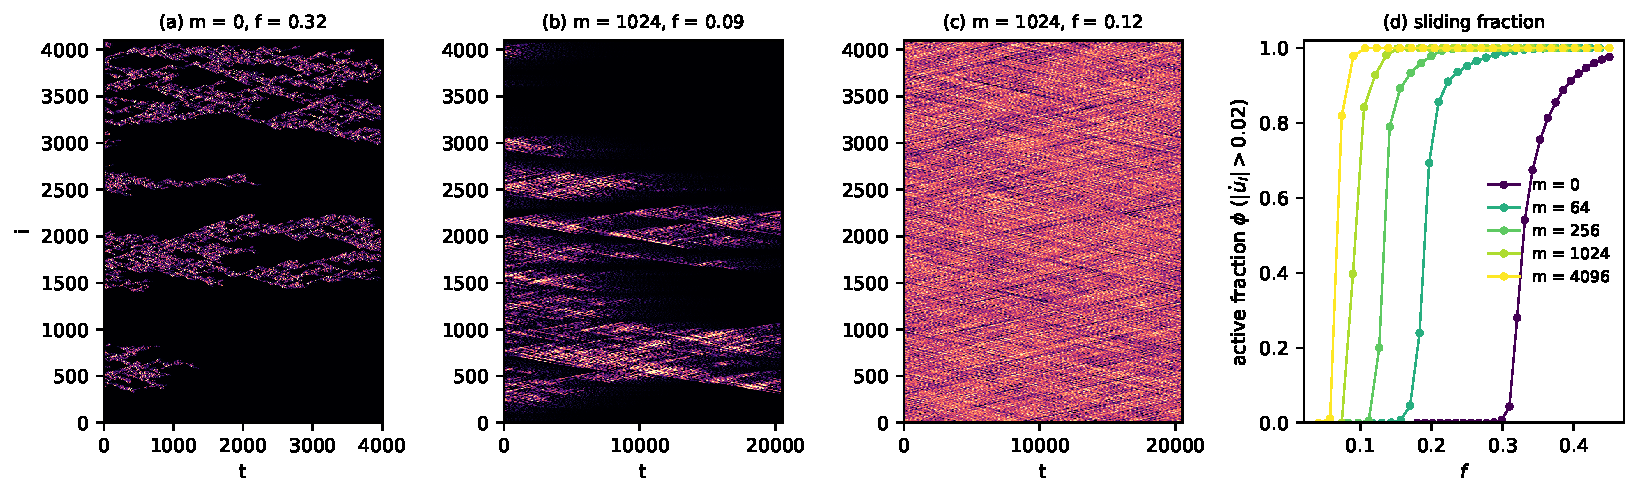
\includegraphics[width=\textwidth]{coexistence.pdf}
\caption{Velocity $\dot u_i(t)$, $L=4096$, blocks of 4 sites. (a) $m=0$ just above $\fcs$: qEW avalanches. (b) $m=1024$, $f=0.09<f_{\min}=0.094$: sliding domains in a pinned line. (c) $m=1024$, $f=0.12$: uniform hot sliding. (d) Active fraction against $f$.}
\label{fig:coex}
\end{figure}

\begin{figure}[H]
\centering
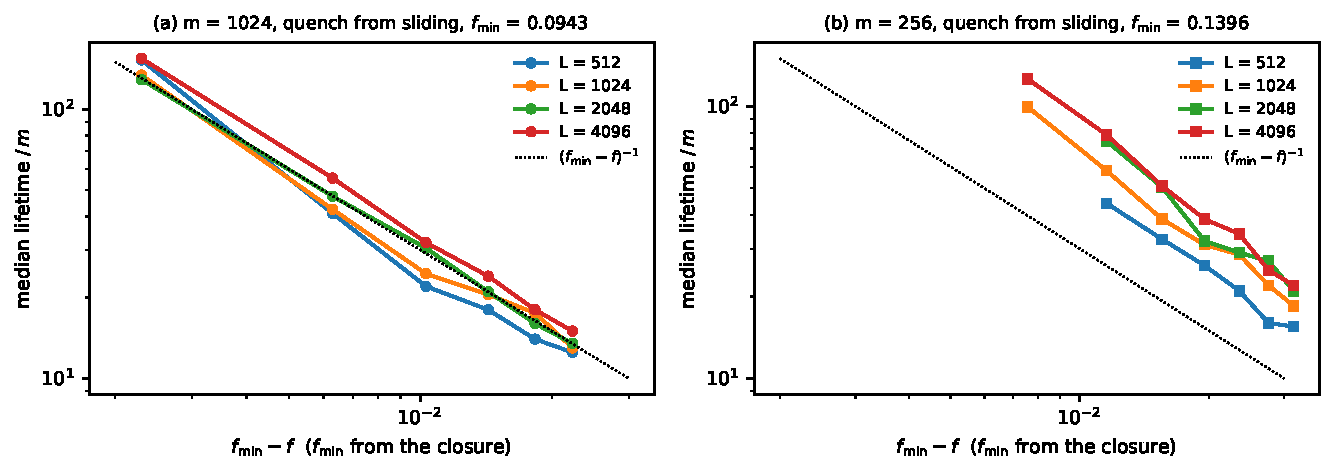
\includegraphics[width=0.85\textwidth]{lifetimes.pdf}
\caption{Median lifetime ($/m$) of a line quenched below $f_{\min}$, against $f_{\min}-f$. (a) $m=1024$, (b) $m=256$. Dotted: $(f_{\min}-f)^{-1}$.}
\label{fig:life}
\end{figure}

\begin{figure}[H]
\centering
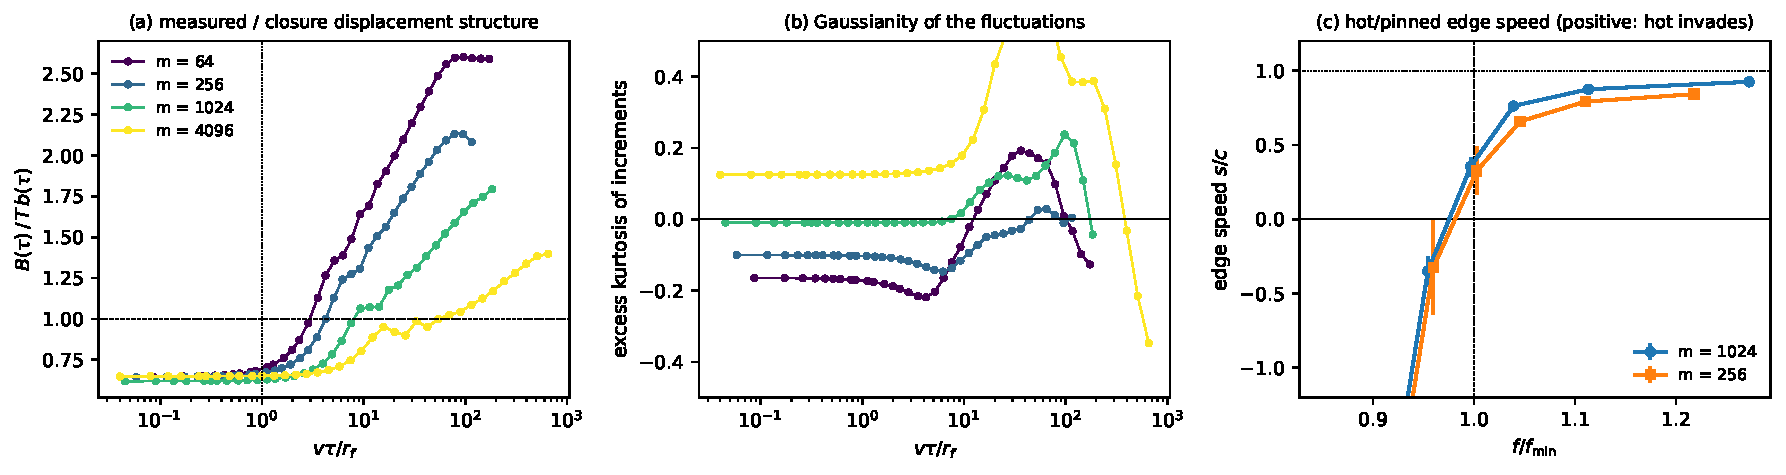
\includegraphics[width=\textwidth]{closure_edges.pdf}
\caption{(a) Measured $B(\tau)$ over the closure's $Tb(\tau)$, against $v\tau/r_f$. (b) Excess kurtosis of increments. (c) Hot/pinned edge speed over $c$, against $f/f_{\min}$ (positive: hot invades).}
\label{fig:edges}
\end{figure}

\begin{figure}[H]
\centering
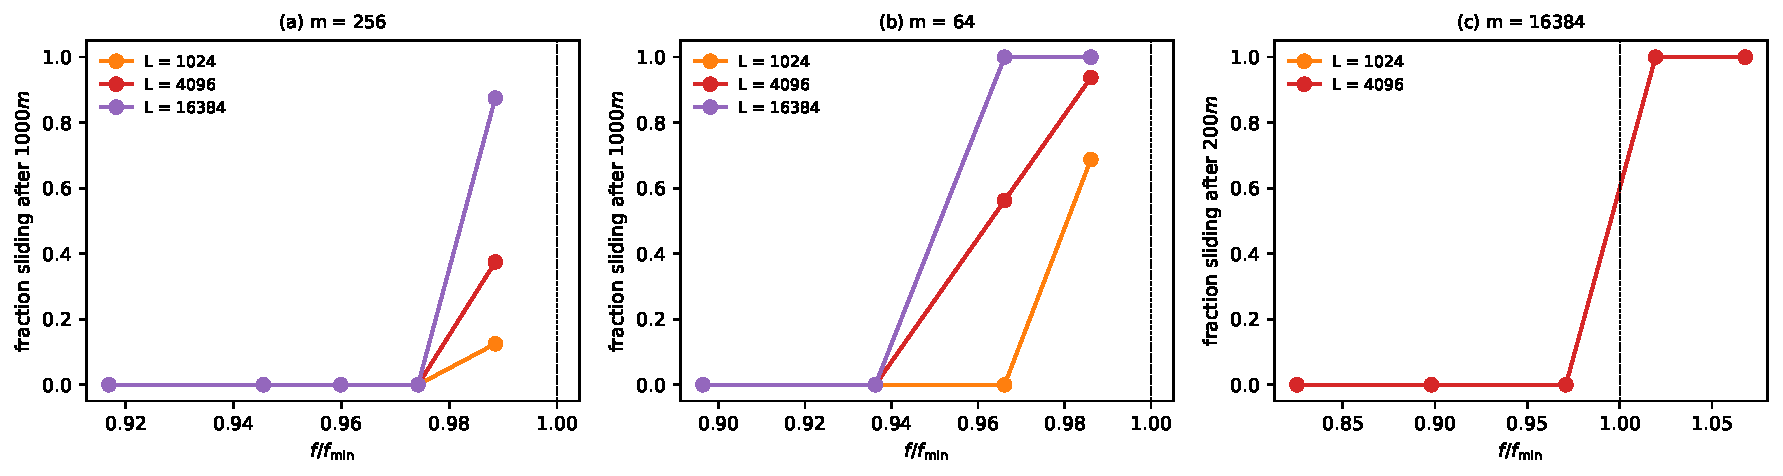
\includegraphics[width=\textwidth]{long_runs.pdf}
\caption{Fraction of quenched lines still sliding at the end of the run, against $f/f_{\min}$. (a) $m=256$, (b) $m=64$ ($1000m$, $L=1024$--16384), (c) $m=16384$ ($200m$).}
\label{fig:gap}
\end{figure}

\subsection{Finite-time thresholds and hysteresis}
\label{sec:finite}

Ramp-down: lower $f$ in steps of $0.0025$ with dwell $\max(1000,10m)$; $\fd$ is where the centre of mass moves less than $0.02$ in the second half of a dwell. Ramp-up: relax at $m=0$, raise $f$ in the same steps each time the line is at rest; $\fu$ is where it travels 30 without stopping. Twelve samples.

\begin{table}[H]
\centering\small
\begin{tabular}{rrcccccc}
\toprule
$m$ & $M$ & $\fd$ & $\fu$ & $f_{\min}$ (closure) & $f_*$ & $\fd/f_*$ & $\fd/f_{\min}$\\
\midrule
0 & 0 & 0.304 & 0.312 & -- & -- & -- & -- \\
1 & 0.37 & 0.301 & 0.312 & -- & 0.667 & -- & -- \\
4 & 1.5 & 0.287 & 0.298 & 0.337 & 0.471 & 0.61 & -- \\
16 & 5.9 & 0.236 & 0.253 & 0.274 & 0.333 & 0.71 & 0.86 \\
64 & 23 & 0.169 & 0.191 & 0.201 & 0.236 & 0.72 & 0.84 \\
256 & 94 & 0.118 & 0.140 & 0.140 & 0.167 & 0.71 & 0.84 \\
1024 & 376 & 0.080 & 0.107 & 0.094 & 0.118 & 0.68 & 0.85 \\
4096 & 1503 & 0.053 & 0.088 & 0.063 & 0.083 & 0.64 & 0.85 \\
\bottomrule
\end{tabular}
\caption{Finite-time thresholds, RF, $L=4096$, standard errors $\le0.0015$; $\fcs\simeq0.308$.}
\label{tab:thr}
\end{table}

\begin{itemize}
\item $\fd/f_{\min}=0.85\pm0.01$ for all $m\ge16$: set by the dwell time (lifetimes of order the dwell), not a threshold.
\item $\fd/\fcs$, $\fu/\fcs$ and $f_{\min}/\fcs$ collapse against $M$ for $A=1$ and $0.5$.
\item The excess hysteresis shrinks as $\sim L^{-1/2}$ for $m\ge256$ ($0.069$, $0.040$, $0.020$ for $L=256$, 1024, 4096 at $m=1024$). On ramp-up the line depins once an avalanche nucleates a surviving hot domain; larger lines nucleate sooner, and $\fu(L)$ falls toward the long-time threshold ($\fu=0.140=f_{\min}$ at $m=256$, $L=4096$).
\end{itemize}

\begin{figure}[H]
\centering
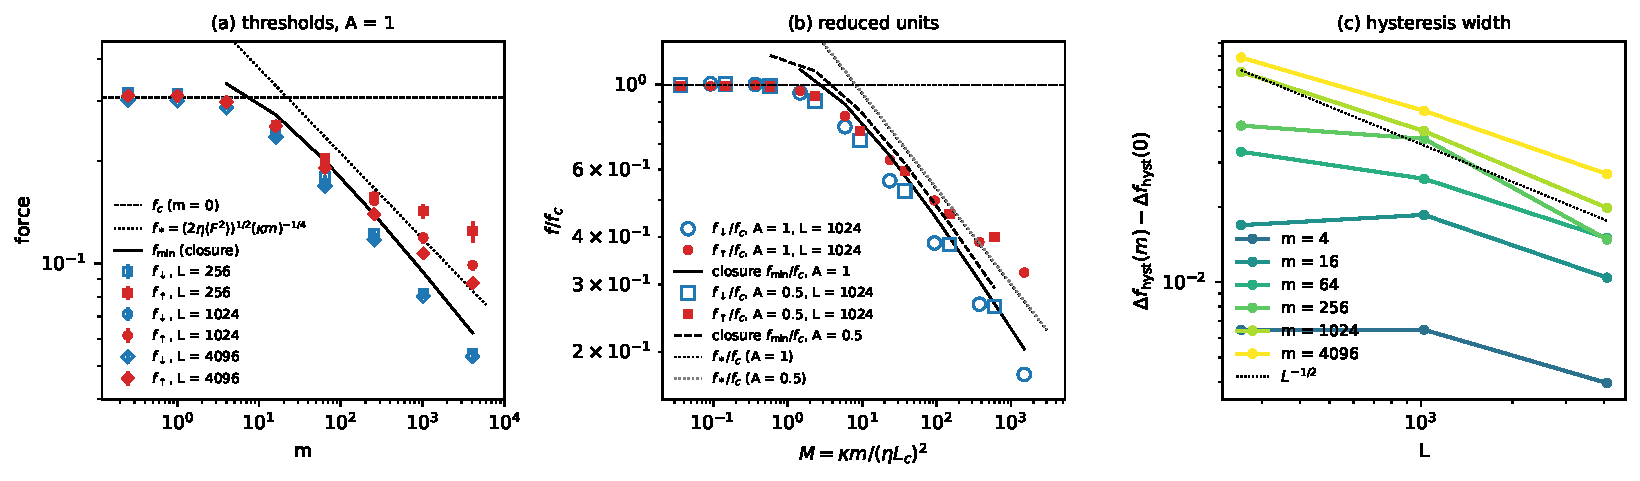
\includegraphics[width=\textwidth]{ramp_thresholds.pdf}
\caption{(a) $\fd$ (open) and $\fu$ (filled) against $m$ for $L=256$, 1024, 4096, with $\fcs$ (dashed), $f_*$ (dotted), closure $f_{\min}$ (solid). (b) Reduced units for $A=1$ and $0.5$ against $M$. (c) Excess hysteresis against $L$.}
\label{fig:thr}
\end{figure}

\subsection{End of sliding at $m=64$: an absorbing-state transition}
\label{sec:patchy}

\paragraph{Field theory.} Near $f_\infty$ hot and pinned regions coexist, so the transition is not perturbative in $\Delta$. The coarse-grained activity $\rho(x,t)$ obeys Reggeon field theory, the field theory of directed percolation (DP), $\mathcal S_{\rm DP}=\int\tilde\rho(\partial_t-D\nabla^2-r+g\rho)\rho-\frac\sigma2\tilde\rho^2\rho$. Three couplings could change the class:
\begin{itemize}
\item \textbf{quenched disorder}, fixed in time: relevant for DP in $d=1$ (Harris, $d\nu_\perp\simeq1.10<2$); MSRJD runs away (Janssen) and strong-disorder RG gives infinite randomness, $\rho\sim(\ln t)^{-0.38}$ with Griffiths phases (Hooyberghs, Igl\'oi, Vanderzande);
\item \textbf{a frozen field}, the pinned configuration left behind: infinitely many absorbing states, with DP stationary exponents and spreading that depends on the absorbing state (Mu\~noz, Grinstein, Dickman, Livi);
\item \textbf{a conserved field}: under constant force $\int\kappa\nabla^2u=0$, so the stress is conserved; coupling to it gives conserved DP, which in $d=1$ maps onto qEW.
\end{itemize}
The exponent that separates DP from conserved DP is $z$: $1.58$ against $1.39$--$1.43$, measured by spreading through $R^2\sim t^{2/z}$.

\paragraph{Where activity dies} ($f_{\min}=0.2008$). Fixed-time survival ($2000m$, $L=16384$, \texttt{runs/patchy.py}) puts patchy sliding down to $0.96f_{\min}$:
\begin{center}\small
\begin{tabular}{cccc}
\toprule
$f/f_{\min}$ & sliding after $2000m$ & $\bar v$ (survivors) & active fraction \\
\midrule
$\le0.956$ & 0 & -- & -- \\
0.961 & 6\% & 0.007 & 0.09 \\
0.971 & 69\% & 0.015 & 0.19 \\
0.976 & 100\% & 0.022 & 0.27 \\
0.996 & 100\% & 0.058 & 0.64 \\
1.021 & 100\% & 0.081 & 0.81 \\
\bottomrule
\end{tabular}
\end{center}
These are transients. The decay of $\rho(t)$ averaged over all lines ($L=65536$, up to $12000m$; \texttt{runs/endslide\_t.py}; Fig.~\ref{fig:endslide}a) decides:
\begin{itemize}
\item $0.974$, $0.976f_{\min}$: faster than any power law, decay times $\approx1000m$, $1500m$; every line stops by $11000m$ (one of 12 survives to $12000m$);
\item $0.984f_{\min}$: still bends down (local slope $0.7$ at $3000$--$9000m$);
\item $0.989f_{\min}$: a slow power law, slope $\approx0.10$, no plateau.
\end{itemize}
In small systems only unusually active lines survive, so survivor averages at fixed time cannot tell first order from critical (Fig.~\ref{fig:endslide}b).

\begin{figure}[H]
\centering
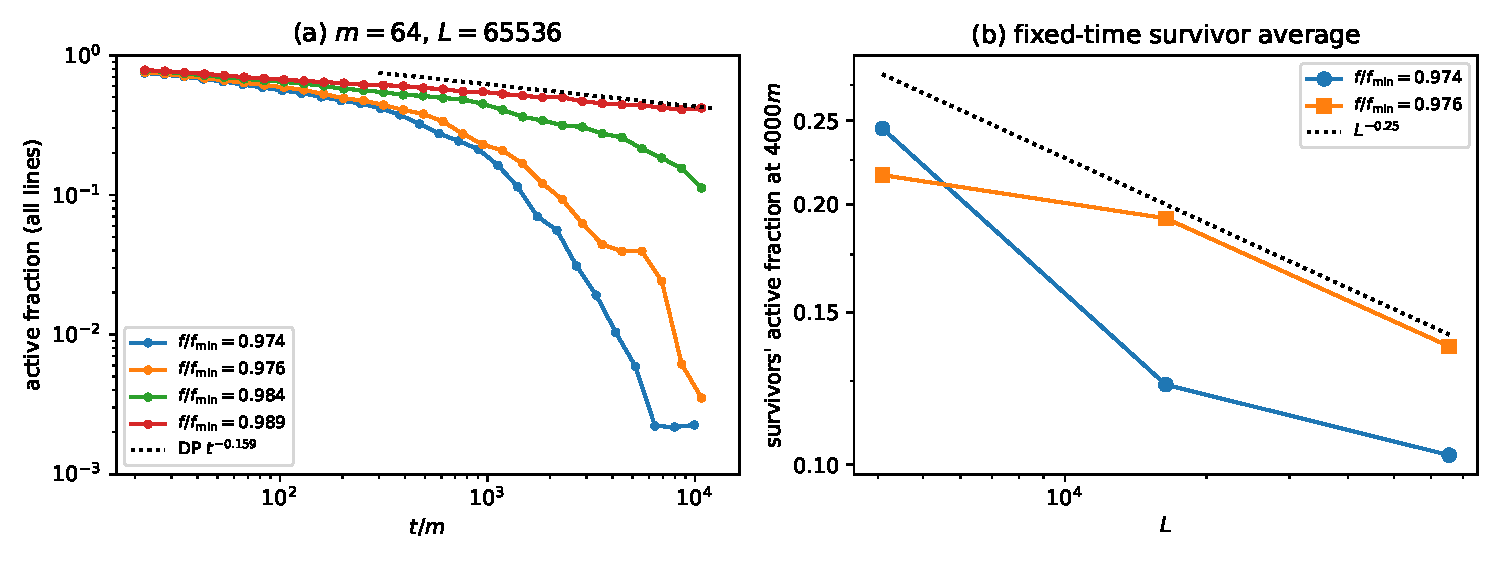
\includegraphics[width=\textwidth]{end_of_sliding.pdf}
\caption{End of sliding at $m=64$. (a) Active fraction averaged over all lines, $L=65536$, 4--6 samples; dotted: DP slope $t^{-0.159}$. (b) Survivors' active fraction after $4000m$ against $L$.}
\label{fig:endslide}
\end{figure}

\paragraph{No quenched rare regions} (\texttt{runs/rare.py}; Fig.~\ref{fig:rare}). Below $f_\infty$ the local slope $-d\ln\rho/d\ln t$ keeps growing ($0.13\to3$--5), with no Griffiths stretch of constant exponent. The long-lived activity of the two lines that outlast the rest is a branching cluster that wanders by $10^4$ sites in $8000m$. Rerun on the same disorder from a line displaced by $37.3$, neither keeps a survivor, and the late activity profiles of the two copies overlap no more than those of different samples. The reason is that the force is random in $u$ as well as in $x$: an active patch keeps advancing into new disorder, so for the activity the disorder is effectively annealed. Infinite randomness is ruled out; DP and conserved DP remain.

\begin{figure}[H]
\centering
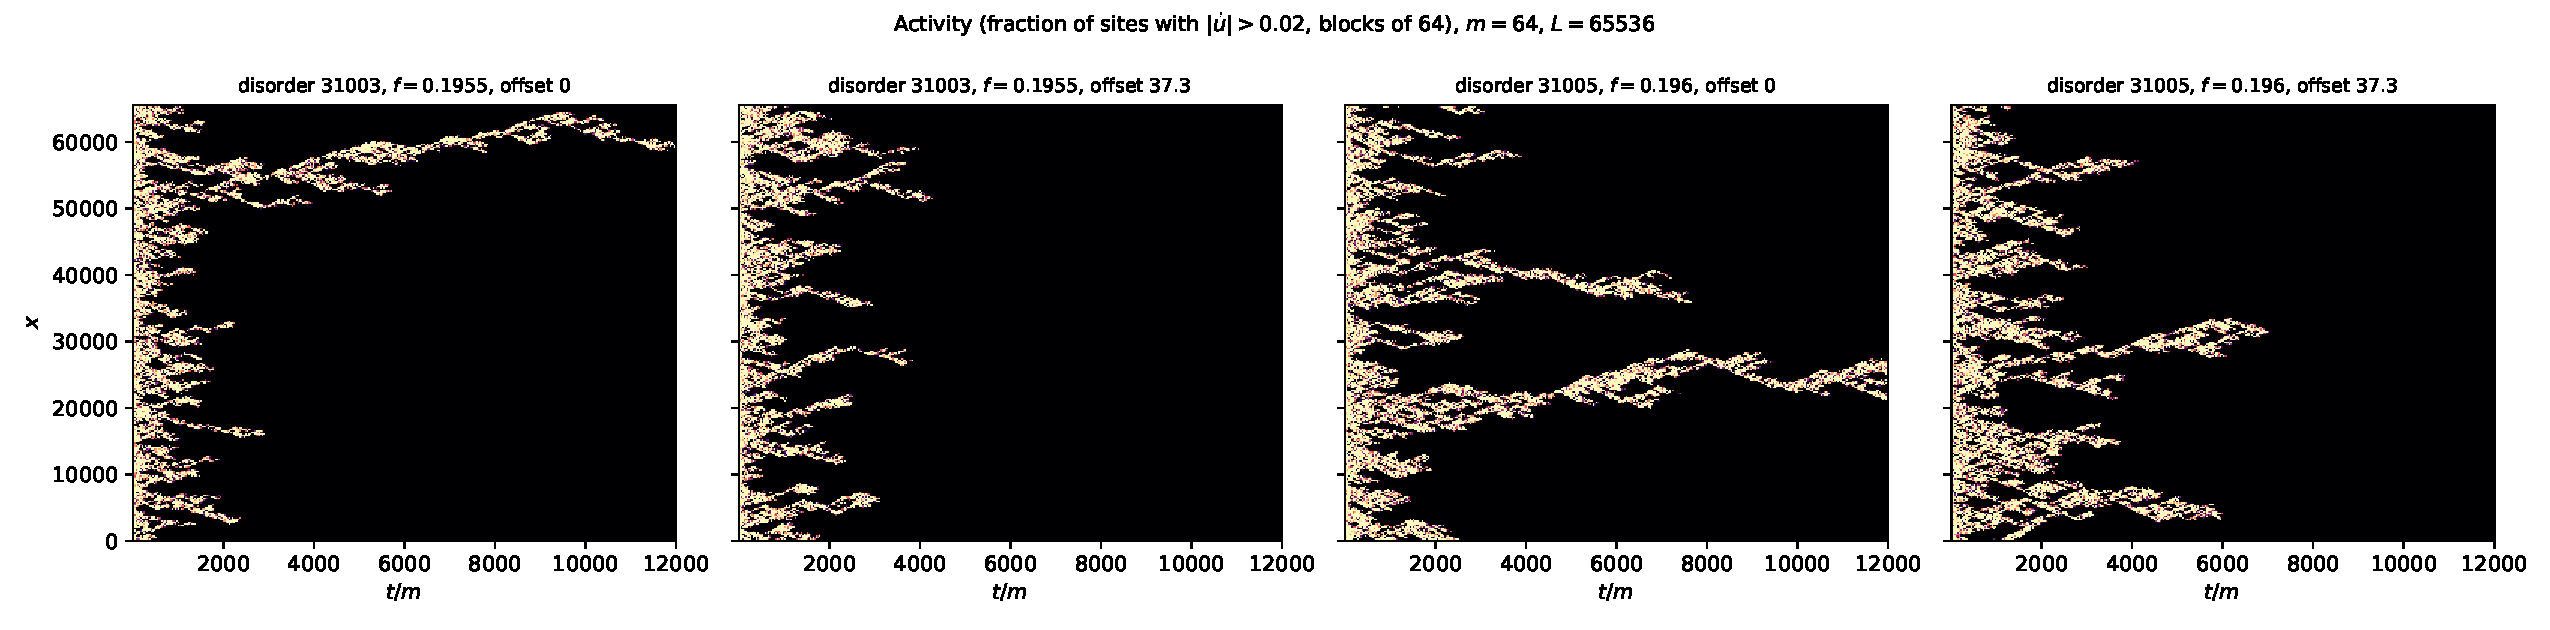
\includegraphics[width=\textwidth]{rare_regions.pdf}
\caption{Activity below $f_\infty$ ($L=65536$, blocks of 64 sites). Each disorder sample is run from two lines differing by a constant displacement. The survivors of the first copy (first and third panels) wander and have no counterpart in the second.}
\label{fig:rare}
\end{figure}

\paragraph{Spreading from a hot seed} (\texttt{runs/spread.py}). Substrates are the natural absorbing state: lines slide at $0.25$, are quenched to $0.974f_{\min}$, and are left until at rest. Each is raised to the test force and kicked (64 sites to velocity $0.3$) at several places, one per copy. Measured: survival $P\sim t^{-\delta}$, active sites $N\sim t^\theta$, spread $R^2\sim t^{2/z}$.
\begin{itemize}
\item \textbf{Critical force} (12 substrates, $L=16384$, 96 runs per force, $2000m$; Fig.~\ref{fig:spread}). At $0.984f_{\min}$ seeds die ($\delta\to0.45$, $\theta<0$); at $0.989f_{\min}$ they invade ($\theta\to0.5$). So $f_\infty=0.1981\pm0.0003=(0.987\pm0.002)f_{\min}$, matching the decay.
\item \textbf{Exponents} (large run: 32 substrates at $L=32768$, 16 kicks each, $5000m$, at $0.1981$ and $0.1983$; the two substrates already active before the kick are dropped, leaving 480 runs per force; bootstrap over substrates; \texttt{analysis/spreading.py}):
\end{itemize}
\begin{center}\small
\begin{tabular}{lccccc}
\toprule
 & DP & conserved DP & window ($m$) & $0.1981$ & $0.1983$ \\
\midrule
$\delta$ & $0.159$ & -- & $100$--$1000$ / $1000$--$5000$ & $0.23\pm0.02$ / $0.20\pm0.03$ & $0.20\pm0.02$ / $0.20\pm0.02$ \\
$\theta$ & $0.313$ & -- & $100$--$1000$ / $1000$--$5000$ & $0.38\pm0.02$ / $0.36\pm0.05$ & $0.44\pm0.03$ / $0.38\pm0.04$ \\
$2/z$ & $1.265$ & $1.40$--$1.44$ & $100$--$1000$ / $1000$--$5000$ & $1.50\pm0.03$ / $1.53\pm0.04$ & $1.51\pm0.03$ / $1.53\pm0.05$ \\
\bottomrule
\end{tabular}
\end{center}
\begin{itemize}
\item \textbf{$z\simeq1.31\pm0.03$ in the largest run.} The local $2/z$ rises from $1.3$ at $30m$ to $\approx1.55$ and stays there out to $5000m$ (Fig.~\ref{fig:spread}d), 7 statistical errors above DP and 3 above conserved DP, at both forces. The 96-run late value ($1.29\pm0.10$) was a fluctuation.
\item \textbf{Systematics} (\texttt{runs/thresholds.py}; Fig.~\ref{fig:thresholds}e; 96 runs each, $f=0.1981$, $[100,1000]m$). The activity threshold does not matter: from $0.0025$ to $0.1$, $\delta$, $\theta$ and $2/z$ move by less than a tenth of their errors. The seed and the substrate do: $2/z=1.47\pm0.07$ (64 sites, $v=0.3$), $1.41\pm0.14$ (16 sites, $v=0.1$), $1.34\pm0.04$ (256 sites), $1.56\pm0.03$ (substrates quenched at $0.95f_{\min}$ instead of $0.974$); $\delta=0.20$--$0.25$, $\theta=0.34$--$0.47$. Every set is above DP; conserved DP is within the spread. A dependence of spreading on the absorbing state is what infinitely many absorbing states predict (Mu\~noz et al.), so part of this spread may be physical rather than pre-asymptotic.
\item \textbf{$\delta$ and $\theta$} lie 1.5--3 errors above DP. Generalized hyperscaling holds: $\theta+2\delta=0.77$--$0.84$ against $1/z=0.75$--$0.79$.
\item \textbf{Reading.} The activity is not carried by short-range contacts: hot edges move at up to the sound speed, and sound carries load ballistically, so spreading is superdiffusive. This is either a separate inertial class, like DP with long-range transport (where $z<1.58$), or a slow crossover if both forces are slightly supercritical. Separating the two needs forces between $0.1975$ and $0.1981$.
\end{itemize}

\begin{figure}[H]
\centering
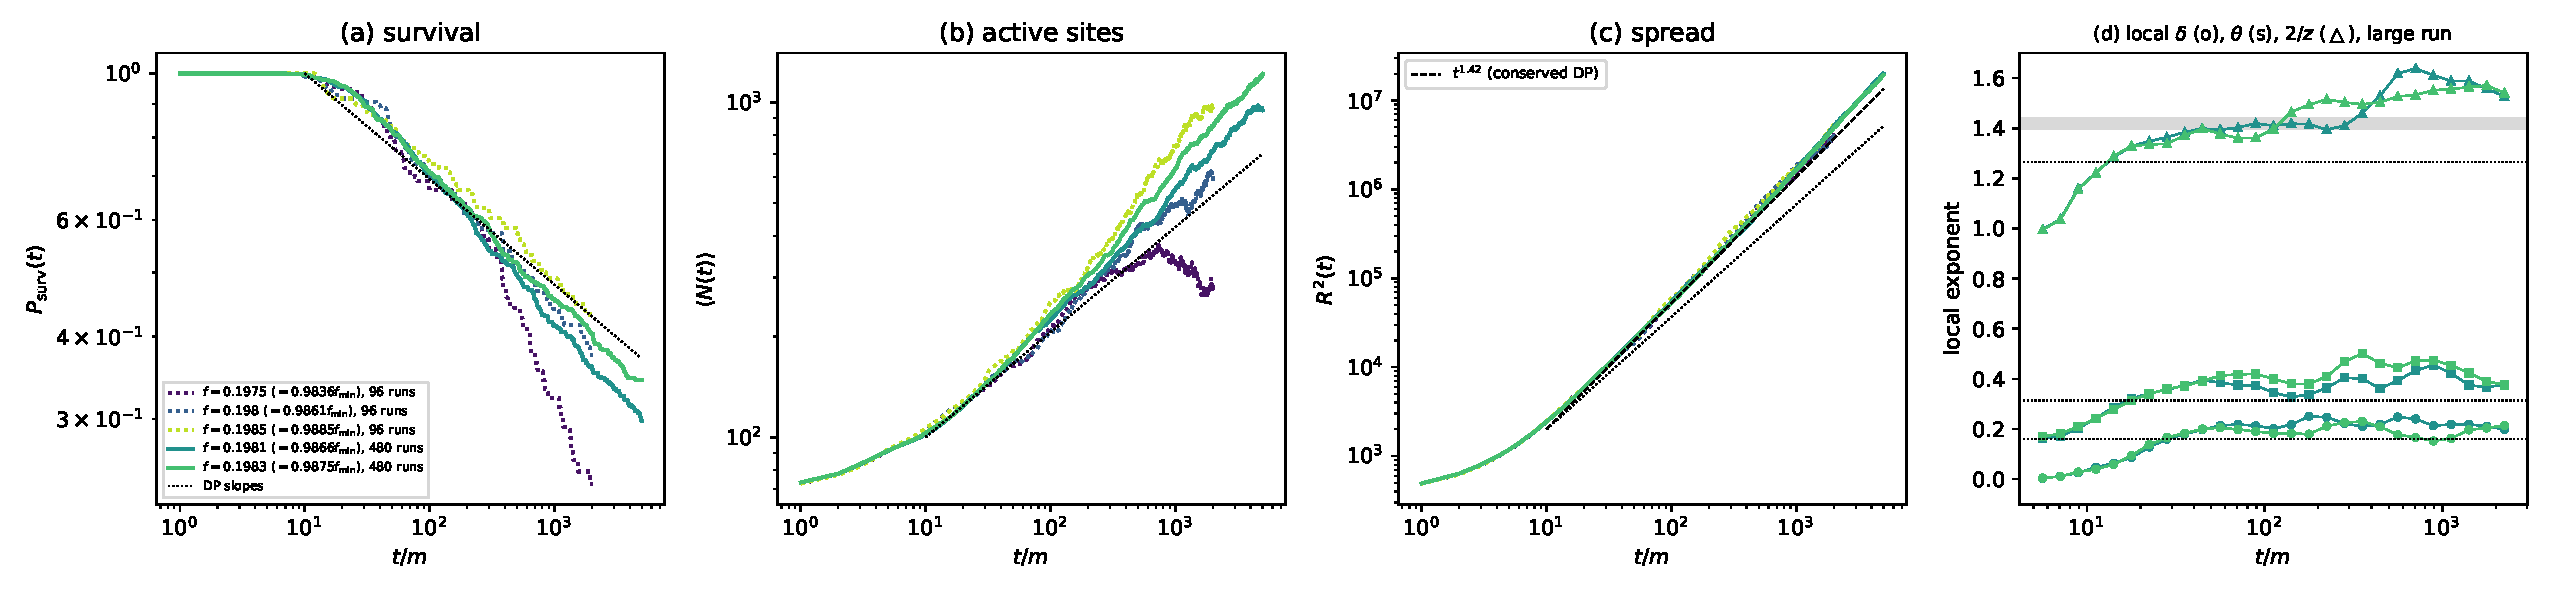
\includegraphics[width=\textwidth]{spreading.pdf}
\caption{Spreading from a hot seed, $m=64$: bracketing run (96 runs, dotted) and large run (480 runs, solid). (a) Survival, (b) mean number of active sites, (c) mean squared spread; dotted: DP slopes, dashed: conserved DP. (d) Local exponents of the large run; dotted: DP values, grey band: conserved-DP $2/z$.}
\label{fig:spread}
\end{figure}

\paragraph{Summary.} The end of sliding at $m=64$ is continuous, at $f_\infty=(0.986$--$0.987)f_{\min}$, with superdiffusive spreading ($z\simeq1.31$, systematic range $2/z=1.34$--$1.57$), consistent with the edge-speed zeros at $m=256$ and 1024 ($0.975$--$0.981f_{\min}$). Patchy sliding between $f_\infty$ and $f_{\min}$ is its active phase (active fraction $0.8\to0.4$). Lifetimes grow to $10^4m$ within 1\% of $f_\infty$, far beyond the $(f_{\min}-f)^{-1}$ law measured lower down: critical slowing down. Pinned regions are not fragile: lines stopped inertially need more extra force to trigger the first avalanche than overdamped-relaxed ones ($0.0019$ against $\lesssim10^{-4}$ at $m=64$; \texttt{runs/marginality.py}), because inertia skips shallow minima.

\subsection{Front models (negative result)}

A deterministic coarse-grained front with the closure friction (\texttt{archive/front\_model.py}) gets the edge-speed saturation near $c$ but ends sliding by a jump at $1.07f_{\min}$. A stochastic block version with local temperatures and self-generated noise (\texttt{archive/front\_model\_stoch.py}) reproduces the closure $f_{\min}$ to 0.1\% and lowers the zero of $s$ to $1.03$--$1.05f_{\min}$, but the end stays a jump above $f_{\min}$. A continuous end below $f_{\min}$ needs heterogeneity between patches, which block averaging removes.

%======================================================================
\section{Small mass: when inertia is irrelevant}
\label{sec:small}

\paragraph{Functional RG.} At the qEW fixed point ($x\to bx$, $t\to b^zt$) the ratio of inertial to viscous terms scales as $M(L_c/\ell)^z$: the mass is irrelevant with eigenvalue $-z$. At one loop the flow of $\Delta$ involves the response only through $\int_0^\infty R_q\,dt=1/\lambda_q$, independent of $m$. So $\zeta\simeq1.25$, $z\simeq1.43$, $\tau=2-2/(1+\zeta)\simeq1.11$, with avalanches smaller than $s_*\sim(L_cM^{1/z})^{1+\zeta}$ inertial. The expansion needs $\dot u\ge0$: for the cusp ($\mathrm{sgn}(u_t-u_{t'})=\mathrm{sgn}(t-t')$), for the exact mean-field instanton, and for no-passing. What breaks it is not the loss of positivity of the response but an overshoot that lands the line in a different metastable state, a finite-amplitude effect. Below that point the line visits the same states as at $m=0$ and everything is qEW. Above it the stopping force shifts, which no loop expansion sees.

\paragraph{Where the shift starts} (24 samples, paired across $m$, $L=2048$; Fig.~\ref{fig:cross}).
\begin{itemize}
\item \textbf{RF:} no shift up to $m=1$; onset at $m\approx1.3$ ($M\approx0.5$, the Larkin-scale mode becoming underdamped, $\ell_m\approx1.4L_c$); then $1.2\%$, $5.3\%$, $11.6\%$, $21\%$ at $m=2$, 4, 8, 16, joining the hot-branch regime without a kink.
\item \textbf{RB:} earlier and steeper ($0.6\%$, $2.1\%$, $6.7\%$, $11\%$ at $m=0.5$, 1, 2, 3), because its wells are stiffer. The onset is set by the microscopic well stiffness and is not universal.
\item \textbf{Same states:} under slow driving, 86\% of the $m=0$ avalanches with $s>10$ recur at $m=1$ at the same position with the same size to 2\%; at $m=2$ only 34\% do (Sec.~\ref{sec:tau}).
\end{itemize}

\begin{figure}[H]
\centering
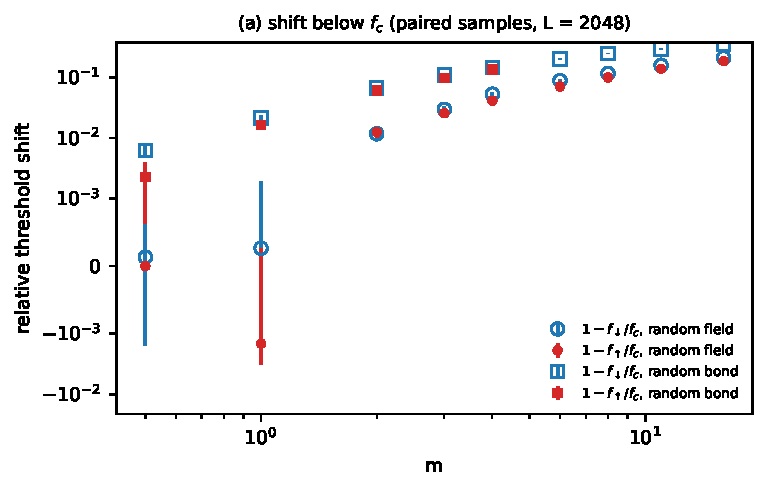
\includegraphics[width=0.55\textwidth]{crossover.pdf}
\caption{Relative shift of $\fd$ (open) and $\fu$ (filled) below $\fcs$, paired samples, RF (circles) and RB (squares).}
\label{fig:cross}
\end{figure}

%======================================================================
\section{Slow driving: stick--slip and avalanches}
\label{sec:slow}

\subsection{Well driving}\label{sec:well}

$k_0=0.01$, $\dot w=10^{-3}$, $L=1024$ (Fig.~\ref{fig:well}). $m=0$: the force fluctuates narrowly around $0.22$ (below $\fcs$, since the well cuts correlations at $k_0^{-1/2}=10$ sites). $m=64$: mean $0.165$. $m=1024$: quasi-periodic stick--slip, loading to $0.12$--$0.17$ and unloading by hot slips to $0.05$--$0.09$, around $f_{\min}=0.094$.

\begin{figure}[H]
\centering
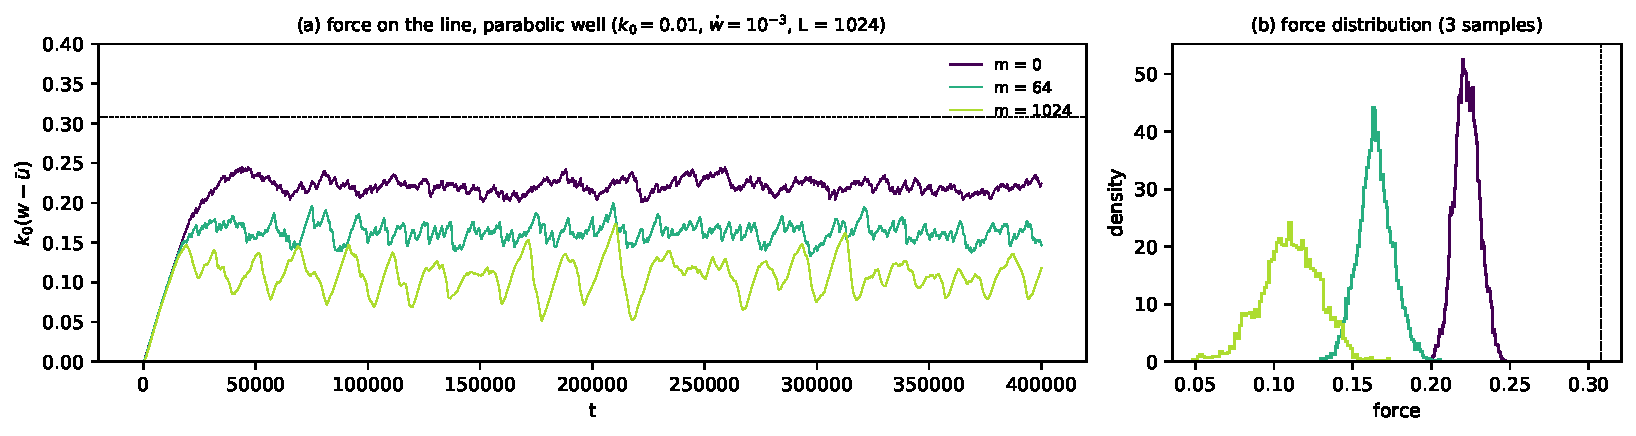
\includegraphics[width=\textwidth]{well_driving.pdf}
\caption{(a) Force $k_0(w-\bar u)$ under slow displacement driving, one sample per mass. (b) Its distribution, 3 samples. Dashed: $\fcs$.}
\label{fig:well}
\end{figure}

\subsection{Avalanches and slips}
\label{sec:aval}

$k_0=3\times10^{-3}$ ($\xi=k_0^{-1/2}\simeq18$), $L=512$, 12 samples, $\dot w=10^{-5}$ after fast loading. An avalanche is an interval with $\bar v>3\dot w$, size $s=L\int(\bar v-\dot w)dt$; ringing fragments closer than $4m$ are merged (\texttt{runs/aval.py}, \texttt{src/aval\_merge.py}; Fig.~\ref{fig:aval}).
\begin{itemize}
\item \textbf{$M\lesssim0.4$:} $m=1$ gives the same avalanches as $m=0$, event for event, and the same mean force ($0.260$).
\item \textbf{$M\gtrsim6$: bimodal.} Cold avalanches, cut off more sharply as $m$ grows, plus slips, events larger than any at $m=0$ ($s>8L$), moving every site by $9.4$, $11.6$, $17$, $29$ (median, $m=16$, 64, 256, 1024) and carrying $15$, $56$, $81$, $88\%$ of the advance. The slip share depends on this definition at intermediate $m$, where $P(s)$ overlaps the qEW tail ($52$, $80$, $91$, $91\%$ for $s>4L$); the forces below change by $<3\%$.
\item \textbf{Slips are a spring block on the hot branch.} A block pulled through kinetic friction $f_k$ slips from $f_{\rm on}$ to $2f_k-f_{\rm on}$; $f_k=(f_{\rm on}+f_{\rm stop})/2=0.90$, $0.98$, $1.10f_{\min}$ at $m=64$, 256, 1024. Arrest at $0.82$, $0.76$, $0.61f_{\min}$.
\item \textbf{Overloading.} Slips start at $0.99$, $1.20$, $1.59f_{\min}$: a slip needs a hot nucleus of size $\sim\ell_m$, while cold avalanches shrink with $m$. The mean force falls from $0.260$ to $0.180$, $0.139$, $0.107$ ($m=64$, 256, 1024), close to $f_{\min}$.
\end{itemize}

\paragraph{Slips are king avalanches.} Events outside the power law of the small ones, spanning the system and carrying most of the advance, are called king avalanches; inertia, stress overshoot, viscoelasticity, internal relaxation and facilitation are all proposed causes (see Sec.~\ref{sec:lit}). Here the inertial mechanism is explicit:
\begin{itemize}
\item \textbf{What a king is:} a stretch of uniform hot sliding. During a slip the line follows the hot branch and the force relaxes as for a block with kinetic friction $f_k\simeq f_{\min}$.
\item \textbf{Why it exists:} the hot branch is non-monotonic (velocity weakening). Once a hot domain survives, the force needed to keep it sliding drops to $f_{\min}$, below the force that started it, so it runs through the whole system.
\item \textbf{Why it is overloaded:} it needs a hot nucleus of size $\sim\ell_m$, which ordinary avalanches reach only at forces up to $1.59f_{\min}$; the overload grows with $m$ because $\ell_m\propto\sqrt m$ while ordinary avalanches shrink.
\item \textbf{Where it starts:} at $M\gtrsim6$ for $\xi\simeq18$; at $M\approx1.5$--6 already for $\xi\simeq45$ (Sec.~\ref{sec:tau}, events larger than $L$ carry 77--90\% of the advance). Whether every $M>0.5$ ends with kings as $\xi\to\infty$ is open problem~\ref{op:xi}.
\item \textbf{Not measured:} the $L$-dependence of the slip size (one $L$ per mass), and the distribution of waiting times between slips; at $m=1024$ under stiffer driving the slips are quasi-periodic (Sec.~\ref{sec:well}).
\end{itemize}

\begin{figure}[H]
\centering
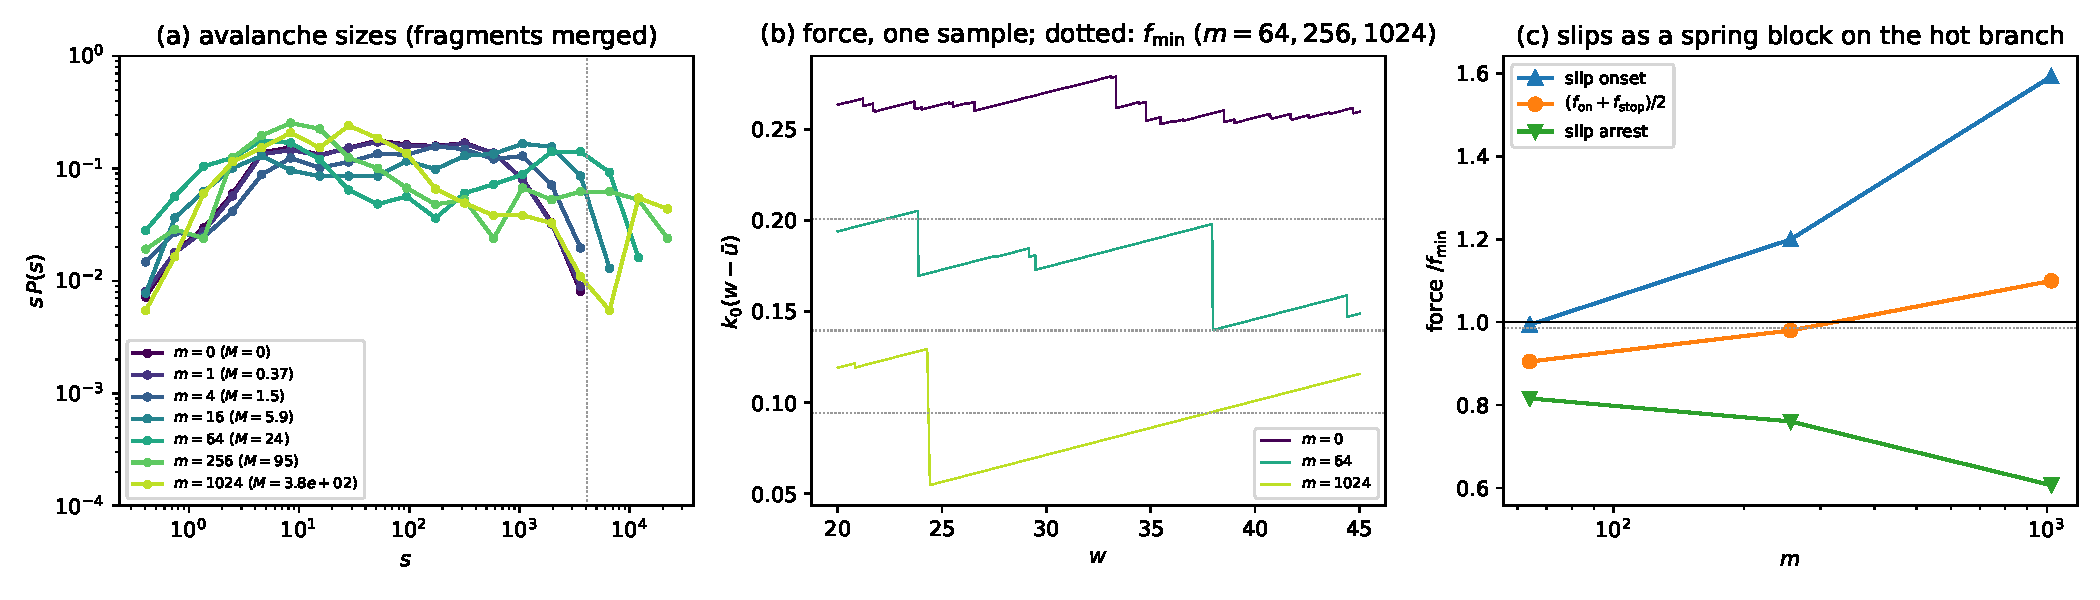
\includegraphics[width=\textwidth]{avalanches.pdf}
\caption{Slow well driving, $k_0=3\times10^{-3}$, $L=512$. (a) Size distributions (fragments merged); dotted: largest avalanche at $m=0$. (b) Force against well position, one sample. (c) Onset, arrest and their mean for slips (larger than any event at $m=0$), over $f_{\min}$; dotted: $f_\infty$.}
\label{fig:aval}
\end{figure}

\subsection{Avalanche exponents}
\label{sec:tau}

Softer well: $k_0=5\times10^{-4}$ ($\xi\simeq45$), $L=2048$, 12 samples, $\sim10^3$ events per mass (\texttt{runs/aval.py tau}, \texttt{analysis/tau.py}; Fig.~\ref{fig:tau}).
\begin{itemize}
\item \textbf{A direct fit is biased.} $s^\tau P(s)$ rises by about two just below the cutoff (the bump of the cutoff function), and $s^{-\tau}e^{-s/s_c}$ then returns $\tau=0.98$, although the same fitter recovers $1.115\pm0.011$ on synthetic data with $1.11$.
\item \textbf{$\tau$ at $m=0$, 1:} pure power law on $3\le s\le300$, $1.06\pm0.03$; moment relation $\langle s\rangle\propto S_m^{2-\tau}$ between the two wells, $1.17\pm0.04$ (detected events) and $1.09$ (sum rule, counting the 15\% of creep below threshold). So $\tau=1.1\pm0.05$, consistent with qEW. Also $s\sim T^{1.6\text{--}1.7}$ (qEW $1.57$) and $\zeta_{\rm eff}=0.96$ from $S_m\propto\xi^{1+\zeta}$ (pre-asymptotic at $\xi\le45$).
\item \textbf{Above the onset inertia matters more at larger $\xi$.} The mean force falls below its $m=0$ value by $0.006$ ($m=4$) and $0.034$ ($m=16$) at $\xi\simeq18$, by $0.007$ and $0.044$ at $\xi\simeq45$, while the $m=0$ force spread shrinks from $0.009$ to $0.002$: the shift grows from $0.6$ to $3.3$ spreads ($m=4$) and from $3.7$ to $20$ ($m=16$). Events larger than $L$ carry 77\% then 90\% of the advance at $m=4$, and $s\sim T^2$ (inertial fronts) replaces $T^{1.57}$. The crossover to stick--slip moves to smaller $M$ as $\xi$ grows.
\end{itemize}

\begin{figure}[H]
\centering
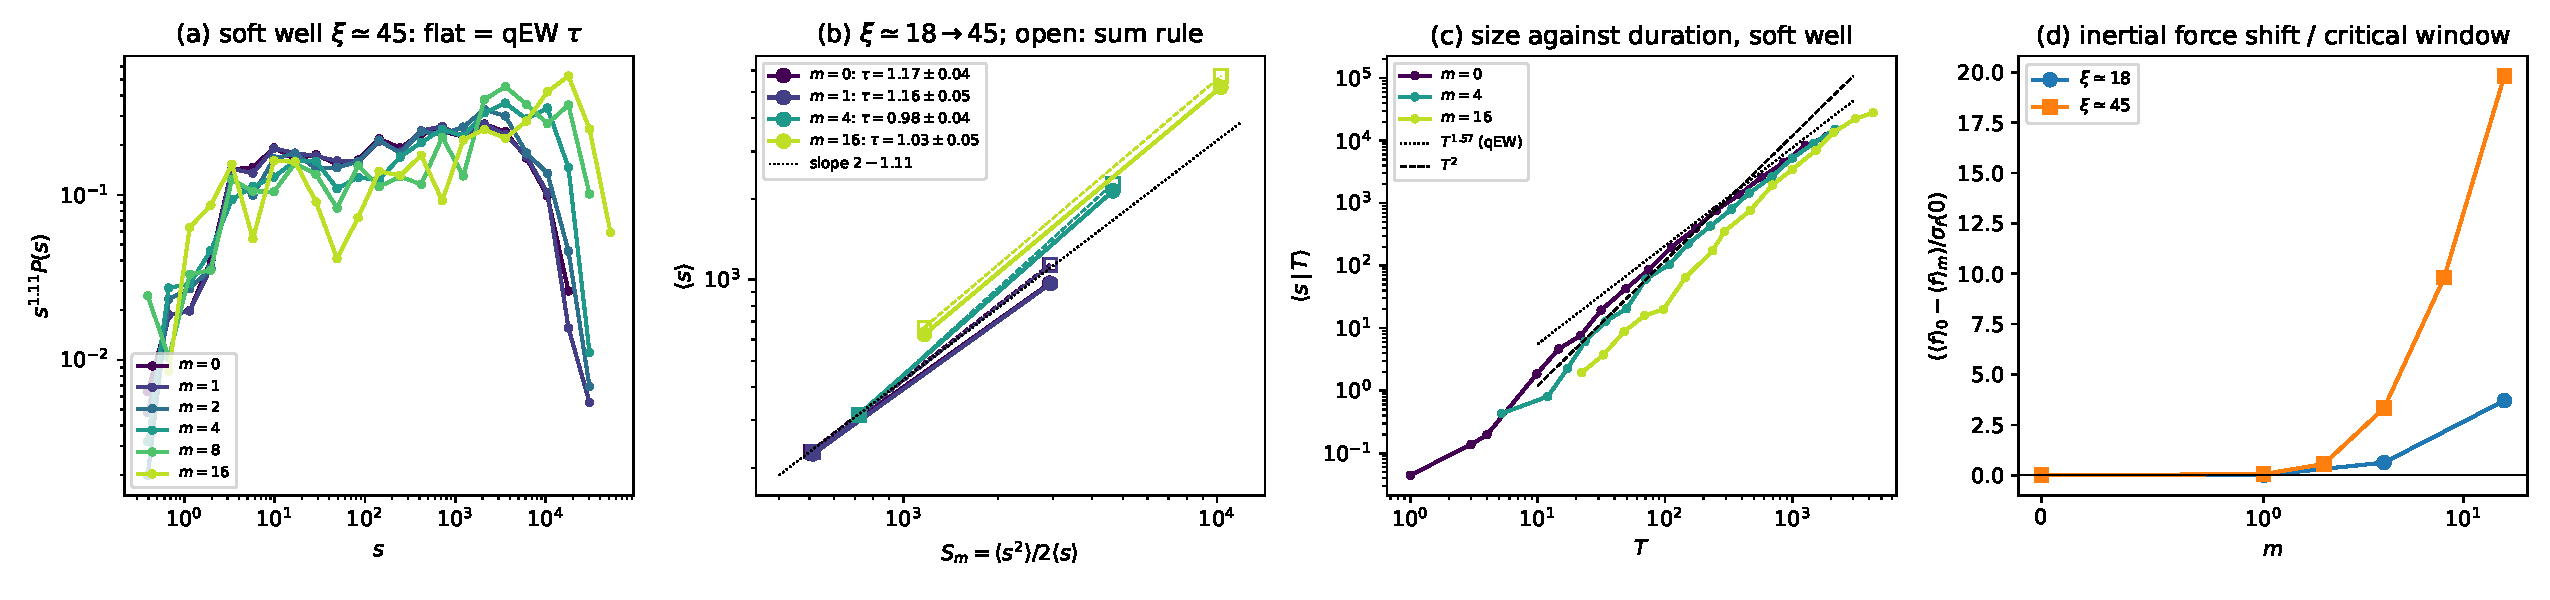
\includegraphics[width=\textwidth]{tau.pdf}
\caption{(a) $s^{1.11}P(s)$, soft well; flat means qEW $\tau$. (b) $\langle s\rangle$ against $S_m$ for $\xi\simeq18$ and $45$ (filled: detected, open: sum rule); dotted: slope $2-1.11$. (c) Mean size at given duration; guides $T^{1.57}$ and $T^2$. (d) Mean-force shift below $m=0$, in units of the $m=0$ force spread.}
\label{fig:tau}
\end{figure}

%======================================================================
\section{Relation to the literature}
\label{sec:lit}

\begin{center}\small
\begin{tabular}{p{2.6cm}p{6.4cm}p{6.6cm}}
\toprule
question & literature & this note \\
\midrule
Does any inertia make depinning first order? & Yes: Fisher (1997, 1998), perturbatively. No for mild inertia: mean field [Schwarz--Fisher 2001, Marchetti 2005], amorphous solids [Salerno et al.\ 2012, Karimi et al.\ 2017]. & No. For $M\lesssim0.5$ the line visits the same states as at $m=0$; threshold, avalanches and $\tau=1.1$ are qEW (Sec.~\ref{sec:small}, \ref{sec:tau}). \\
Where is the crossover? & Not located. de Geus--Wyart (2024) suggest their scenarios B and C hold at different inertia. & At $M\approx0.5$, the onset of overshoot in single jumps; set by the microscopic well stiffness, so not universal (Sec.~\ref{sec:small}). \\
Flow-curve minimum $f_{\min}$ & Mean field: non-monotonic flow curve, tricritical point [Schwarz--Fisher 2001, 2003]. 1D inertial line: $f_{\min}$ measured; ``objectively extracting $f_{\min}$ \ldots\ is currently not possible'' [de Geus--Wyart 2024]. & Computed with no fitted parameters: closure (Sec.~\ref{sec:closure}); whole hot branch from the $\Sigma(\omega)$ DMFT (Sec.~\ref{sec:dmft}); $f_{\min}\propto m^{-3/10}$ (RF), $m^{-5/14}$ (RB) (Sec.~\ref{sec:heavy}). \\
Threshold of a heavy line & $f_c\simeq f_{\min}$, slightly above, nucleated by avalanches; gap unresolved [de Geus--Wyart 2024; rate-and-state, Brener et al.\ 2018]. & $f_\infty=(0.987\pm0.002)f_{\min}$, \emph{below} $f_{\min}$: patchy sliding survives under the minimum (Sec.~\ref{sec:patchy}). \\
Hysteresis at $L,t\to\infty$ & Finite: one-way hysteresis generic in overshoot automata [Maimon--Schwarz 2004]; tiny but finite [de Geus--Wyart 2024]. & None measurable: ramp hysteresis shrinks as $L^{-1/2}$ and with dwell time (Sec.~\ref{sec:finite}). \\
Order of the transition & Continuous with hysteresis [Maimon--Schwarz 2004]; first-order-like, flow nucleates at finite speed [de Geus--Wyart 2024]. & Uniform sliding ends at $f_{\min}$ with finite $v$; the patchy state ends continuously at $f_\infty$, an absorbing-state transition with no rare regions. \\
Avalanches with inertia & New underdamped class [Salerno et al.\ 2012, 2013]; small events keep the overdamped statistics [Karimi et al.\ 2017]; characteristic events from dynamic weakening [Fisher et al.\ 1997]; king avalanches with inertia, overshoot, viscoelasticity or aging as proposed causes [arXiv:2604.13222 (2026) and refs.\ therein]. & Small $M$: qEW, $\tau=1.1$. $M\gtrsim6$: king avalanches = slips along the hot branch, kinetic friction $\simeq f_{\min}$, nucleus $\sim\ell_m$ (Sec.~\ref{sec:aval}). No long-range kernel here, so their exponents are not directly comparable. \\
Hot sliding state & Shaking temperature $\propto\hat\Delta(0)/v$ [Koshelev--Vinokur 1994; Giamarchi--Le Doussal 1996]; overdamped DMFT of driven disordered systems [Horner 1996; Cugliandolo et al.\ 1997]; inertial ABBM, one degree of freedom [Le Doussal et al.\ 2012]. & The bare $S_\xi(0)$ is the shaking temperature; self-consistent smearing raises it by 2--2.5, $S_\xi(0)=\hat\Delta(0)/((1-H)v)$. Underdamped, energy-conserving DMFT with $\Sigma(\omega)$ (Sec.~\ref{sec:dmft}). \\
Spreading class & DP for short-range absorbing transitions (Janssen--Grassberger); conserved DP $\equiv$ qEW [Le Doussal--Wiese 2015]; L\'evy-flight DP [Janssen et al.\ 1999]; sound-carried stress in crack fronts [Ramanathan--Fisher 1997]. & $z\simeq1.31\pm0.03$ (largest run; $2/z=1.34$--$1.57$ across seeds and substrates), faster than DP ($1.58$); conserved DP ($1.43$) within the spread: consistent with long-range, L\'evy-like transport (Sec.~\ref{sec:patchy}). \\
\bottomrule
\end{tabular}
\end{center}

\paragraph{Agreement.} Weak inertia is irrelevant (scenario B of de Geus--Wyart), and strong inertia gives characteristic slip events whose kinetic friction is the flow-curve minimum. The mean-field picture is reproduced by the DMFT: its uniform branch is non-monotonic, as in Schwarz--Fisher.

\paragraph{New.} (i) $f_{\min}$ and the whole hot branch are computed, not measured. (ii) The crossover to inertial behaviour is located at $M\approx0.5$ and traced to single-jump overshoot. (iii) The long-time threshold is resolved and lies below $f_{\min}$; the end of sliding is continuous, not the spinodal of the mean-field branch. (iv) The spreading class is not DP.

\paragraph{Tension.} de Geus--Wyart find $f_c\gtrsim f_{\min}$ with finite hysteresis; we find $f_\infty<f_{\min}$ and none. The protocols differ: their $f_c$ is the lowest force at which avalanches triggered in a \emph{pinned} line span the system; our $f_\infty$ is where a \emph{sliding} line stops. A pinned line may need $f\gtrsim f_{\min}$ to start while a sliding one only stops below $f_{\min}$; that would be hysteresis between the two protocols, which our ramps bound as finite-size. Their model also differs (parabolic-well disorder, anharmonic elasticity, $\eta=0.1$, $m=1$). Running both protocols on one model settles it (open problem~\ref{op:protocol}).

\paragraph{References.}
{\footnotesize
Brener, Aldam, Barras, Scheibert, Bouchbinder, PRL 121, 234302 (2018).
Cugliandolo, Kurchan, Le Doussal, Peliti, PRL 78, 350 (1997).
Ferrero, Bustingorry, Kolton, PRE 87, 032122 (2013).
de Geus, Wyart, PRE 106, 065001 (2022), arXiv:2204.02795; arXiv:2411.06732 (2024).
Fisher, Phys.\ Rep.\ 301, 113 (1998).
Fisher, Dahmen, Ramanathan, Ben-Zion, PRL 78, 4885 (1997).
Giamarchi, Le Doussal, PRL 76, 3408 (1996).
Horner, Z.\ Phys.\ B (1996).
Janssen, Oerding, van Wijland, Hilhorst, Eur.\ Phys.\ J.\ B 7, 137 (1999).
Karimi, Ferrero, Barrat, PRE 95, 013003 (2017), arXiv:1610.00533.
Koshelev, Vinokur, PRL 73, 3580 (1994).
Le Doussal, Petkovi\'c, Wiese, PRE 85, 061116 (2012).
Le Doussal, Wiese, PRL 114, 110601 (2015).
Maimon, Schwarz, PRL 92, 255502 (2004), arXiv:cond-mat/0301495.
Marchetti, arXiv:cond-mat/0503639 (2005).
Middleton, PRL 68, 670 (1992).
Global oscillations in depinning models with aging, arXiv:2604.13222 (2026).
Ramanathan, Fisher, PRL 79, 877 (1997).
Salerno, Maloney, Robbins, PRL 109, 105703 (2012); Salerno, Robbins, PRE 88, 062206 (2013).
Schwarz, Fisher, PRL 87, 096107 (2001); PRE 67, 021603 (2003).
Journal volumes not marked with an arXiv number are from memory and should be checked before citing.
}

%======================================================================
\section{Open problems}

\begin{enumerate}
\item \textbf{The class of the end of sliding.} Spreading gives $z\simeq1.31\pm0.03$ in the largest run, but $2/z$ varies from $1.34$ to $1.57$ with the seed and the substrate: DP is excluded, conserved DP is not. Larger runs with several seeds and substrates, out to $10^4m$, are needed to tell whether the spread is pre-asymptotic or a real dependence on the absorbing state. Forces between $0.1975$ and $0.1981$ would separate a slightly supercritical crossover from a separate inertial class with long-range (sound-carried) transport, and $\rho(t)$ at $f_\infty$ over three decades would give $\delta$ independently.
\item \textbf{A theory of where sliding ends.} The conserving Gaussian DMFT describes uniform hot sliding quantitatively but keeps a stable hot branch below $f_\infty$: the end is not a property of the uniform state. Two routes: (a) the numerical cavity with the $\Sigma(\omega)$ medium, whose exact site can stick, to test whether non-Gaussian sticking alone ends the branch; (b) a spatially resolved theory in which the bath itself can be locally pinned, i.e.\ coexistence.
\item \textbf{A theory of coexistence.} Local theories (closure, DMFT, block front models) end sliding by a jump above $f_{\min}$; the measured end is continuous and below it. A spatially resolved theory of hot and pinned patches is missing.
\item \textbf{Start versus stop.}\label{op:protocol} Measure the lowest force at which avalanches triggered in a pinned heavy line span the system (the de Geus--Wyart $f_c$) at $m=64$ and compare with $f_\infty$ and $f_{\min}$; a gap that survives $L\to\infty$ would be genuine start/stop hysteresis.
\item \textbf{Avalanches at larger $\xi$.}\label{op:xi} Separating $\tau=1.08$ from $1.11$ needs $\xi\gtrsim100$; whether every $M>0.5$ ends in stick--slip as $\xi\to\infty$ needs a series of wells at $m=2$--4.
\end{enumerate}

%======================================================================
\section{Reproduce}
\label{sec:reproduce}

Library code is in \texttt{src/}, production runs in \texttt{runs/} (writing \texttt{data/}), one analysis script per topic in \texttt{analysis/} (writing \texttt{figures/} and \texttt{data/stats/}); superseded and exploratory scripts are in \texttt{archive/}. Scripts can be launched from any directory (they import \texttt{src/config.py}, which moves to the \texttt{inertia} folder); set \texttt{NUMBA\_NUM\_THREADS} to limit the load. Core code: \texttt{src/sim.py} (integrator; $A<0$ selects RB), \texttt{src/protocols.py} (flow, ramps, lifetimes, well), \texttt{src/linresp.py} (second order), \texttt{src/sc.py} (closure).
\begin{center}\small
\begin{tabular}{p{3.4cm}p{12cm}}
\toprule
section & scripts \\
\midrule
\ref{sec:second}, \ref{sec:closure} & \texttt{runs/sliding.py flow}, \texttt{runs/closure\_flow.py}, \texttt{runs/closure\_flow\_rb.py}, \texttt{runs/check\_closure.py}; exploratory \texttt{archive/sc\_noneq.py}, \texttt{archive/sc\_hybrid.py}; \texttt{analysis/sliding.py} (Fig.~\ref{fig:flow}), \texttt{analysis/closure\_crossover.py} (Fig.~\ref{fig:edges}) \\
\ref{sec:dmft} & \texttt{runs/cavity\_runs.py}, \texttt{runs/cavity\_polish.py} (\texttt{src/cavity.py}); \texttt{src/gdmft2.py 1024 0.0891 0.0708 0.0512}, \texttt{src/gdmft2.py 256 0.1169}, \texttt{runs/dmft\_flow.py}; constant-$\eta_{\rm eff}$ version \texttt{src/gdmft.py}, \texttt{archive/gdmft\_flow.py}; \texttt{analysis/single\_site.py} (Fig.~\ref{fig:dmft}), \texttt{analysis/dmft\_flow.py} (Fig.~\ref{fig:dmftflow}) \\
\ref{sec:rough} & \texttt{runs/sq.py run}, \texttt{runs/sq.py theory}, \texttt{runs/sq\_near.py 0.10 0.105 0.11}, \texttt{runs/sq\_diag.py 1024 0.12} (and 1024 0.11, 1024 0.10, 256 0.17); \texttt{analysis/roughness.py} \\
\ref{sec:heavy} & \texttt{runs/lifetimes\_rb.py rb heavy}, \texttt{runs/crossover\_gap.py heavy}; \texttt{analysis/lifetimes\_rb.py} (Fig.~\ref{fig:heavy}) \\
\ref{sec:invasion}, \ref{sec:finite} & \texttt{runs/sliding.py kymo thresholds}, \texttt{runs/lifetimes\_rb.py life}, \texttt{runs/lifetimes\_fmin.py}, \texttt{runs/crossover\_gap.py gap}, \texttt{runs/edges.py 1024 256 64}, \texttt{runs/gap64.py}; \texttt{analysis/sliding.py} (Figs.~\ref{fig:coex}, \ref{fig:thr}), \texttt{analysis/lifetimes\_rb.py} (Fig.~\ref{fig:life}), \texttt{analysis/closure\_crossover.py} (Figs.~\ref{fig:edges}, \ref{fig:gap}) \\
\ref{sec:patchy} & \texttt{runs/patchy.py}, \texttt{runs/marginality.py}, \texttt{runs/endslide.py}, \texttt{runs/endslide\_L.py}, \texttt{runs/endslide\_t.py}, \texttt{runs/endslide\_t.py 0.1975 0.1985}, \texttt{runs/rare.py}, \texttt{runs/spread.py sub}, \texttt{runs/spread.py run 0.198 0.1975 0.1985 --T 2000}, \texttt{SPREAD\_L=32768 SPREAD\_NSUB=32 SPREAD\_NK=16 runs/spread.py sub} and \texttt{runs/spread.py run 0.1981 0.1983 --T 5000}; \texttt{analysis/end\_of\_sliding.py}, \texttt{analysis/rare\_regions.py}, \texttt{archive/analyze9.py}, \texttt{analysis/spreading.py}; exploratory \texttt{archive/front\_model.py}, \texttt{archive/front\_model\_stoch.py} \\
\ref{sec:small} & \texttt{runs/crossover\_gap.py cross}; \texttt{analysis/closure\_crossover.py} \\
\ref{sec:slow} & \texttt{runs/sliding.py well}, \texttt{runs/aval.py scan}, \texttt{runs/aval.py tau}; \texttt{analysis/sliding.py} (Fig.~\ref{fig:well}), \texttt{analysis/avalanches.py}, \texttt{analysis/tau.py} \\
\bottomrule
\end{tabular}
\end{center}

\end{document}
